\documentclass[msc]{ppgccufmg}    

%\usepackage[brazil]{babel}        
\usepackage[english]{babel}     
\usepackage[latin1]{inputenc}
\usepackage[T1]{fontenc}
\usepackage{type1ec}
\usepackage{graphicx}
\usepackage{amsmath}
\usepackage{listings}
\usepackage{float}
\usepackage{adjustbox}
\usepackage{multirow}
\usepackage{color}
\usepackage{courier}
\usepackage[section]{placeins}
\usepackage[a4paper,
  bookmarks=true,
  bookmarksnumbered=true,
  linktocpage,
  colorlinks,
  citecolor=black,
  urlcolor=black,
  linkcolor=black,
  filecolor=black,
  ]{hyperref}
\usepackage[square]{natbib}

\clubpenalty=10000 
\widowpenalty = 10000 

\newcommand{\ts}{\textsuperscript}

\newcommand{\cell}[2][c]{\begin{tabular}[#1]{@{}c@{}}#2\end{tabular}}
\renewcommand{\arraystretch}{1.2}

\floatstyle{ruled}
\newfloat{Listing}{tbp}{loa}


\begin{document}



\ppgccufmg{
  title={An Empirical Study About the Use of Optional Typing in Software Systems},
  authorrev={Garcia de Souza, Carlos Alexandre},
  cutter={D1234p},
  cdu={519.6*82.10},
  university={Federal University of Minas Gerais},
  course={Computer Science},
  address={Belo Horizonte},
  portuguesetitle={Um Estudo Emp\'{i}rico sobre o Uso de Tipagem Opcional em Sistemas de Software},
  portugueseuniversity={Universidade Federal de Minas Gerais},
  portuguesecourse={Ci\^{e}ncia da Computa\c{c}\~{a}o},
  date={2014-03},
  advisor={Eduardo Magno Lages Figueiredo},
  % approval={img/approvalsheet.eps},
  abstract=[brazil]{Resumo}{resumo},
  abstract={Abstract}{abstract},
  dedication={dedicatoria},
  ack={agradecimentos},
%{The truth is rarely pure and never simple.}{Oscar Wilde}
  epigraphtext={If someone claims to have the perfect programming language, he is either a fool or a salesman or both.}{Bjarne Stroustrup},
  keywords={Type Systems, Repository Analysis, Optional Typing, Groovy},
}





\newcommand{\dummytxt}{\dummytxta\dummytxtb\dummytxtc}

\chapter{Introduction}

Type systems are one of the most important characteristics of a programming language and also a major topic of research in software engineering (\cite{Furr09,takikawa12,gradual_typing}).
A type system is a tractable syntactic method for proving the absence of certain program behaviors by classifying phrases according to the kinds of values they compute (\cite{types_and_programming_languages}).
In other words, type systems define the interface of the different parts that compose a program.
Their main purposes are to prevent the occurrence of execution errors and to document code (\cite{type_systems}).
In dynamically typed languages, such as Ruby and JavaScript, the definition of the type of an expression only happens at run time.
On the other hand, statically typed programming languages, such as Java and C\#, require types to be defined during compile time, either explicitly declared by the programmer or inferred by the compiler (\cite{Milner78}).
In such languages, the compiler can check for type errors statically.

Discussions about what is the best type system for a particular situation have become increasingly important in recent years due to the rapid popularization of dynamically typed languages. 
According to the TIOBE Programming Community Index (\cite{tiobe}), a well-known ranking that measures the popularity of programming languages, 27\% of the programming languages used in industry are dynamically typed. 
A decade ago, this number was only 17\%. 
Among the 10 languages on top of the ranking, four are dynamically typed: JavaScript, Perl, Python and PHP. 
None of these languages were among the top 10 rank before 1998.

Several factors may be considered when choosing a typing paradigm. 
Dynamically typed languages tend to allow programmers to code faster and to adapt their programs to frequently changing requirements more easily.
Also, by removing the repetitive work of defining types, these languages allow programmers to focus on the problem to be solved rather than on the rules of the language (\cite{dynamically_typed_languages}).

Statically typed languages also have their advantages. 
They allow compilers to find type errors statically (\cite{should_your_specification_language_be_typed}). 
Typed declarations increase the maintainability of systems because they implicitly document the code, telling programmers about the nature of expressions (\cite{type_systems,mayer2012static}). 
Systems built with these languages tend to be more efficient since they do not need to perform type checking during execution (\cite{Bruce2002,jit}). 
Finally, modern development environments, such as Eclipse and IDEA, are able to assist programmers with functionalities such as code completion based on the information provided by statically typed declarations (\cite{bruch2009learning}).

Some languages try to combine characteristics from both static and dynamic type systems.
\cite{groovy} is one of these languages.
Although Groovy is mostly a dynamically typed language, it gives programmers the option to use type annotations as a means to document their code.
It is also possible to turn static type checking on so the compiler can find type errors before execution.
This allows developers to choose the most appropriate paradigm for each situation.


\section{Motivation}
Although the tradeoffs between different typing paradigms have been widely researched, specially though controlled experiments, it is still unclear how programmers actually perceive these tradeoffs.
For example, assuming that typed programs are more reliable, but untyped programs can be written faster, which factor would be considered more relevant by programmers and in which contexts?

Understanding the point of view of programmers about the use of types is an important matter.
Programming language developers can consider this information in their design so they can develop the most appropriate features for their target audience.
Tools can be created or improved to overcome weaknesses of languages. 
Finally, programmers can benefit from this knowledge when choosing programming languages or typing paradigms for a given context.

Finding the programmers' point of view about the use of types is far from trivial.
Controlled experiments hardly reproduce real life situations, where many experienced programmers interact through a long period of time to build large and complex software systems \cite{Wohlin2012}.
Also, one can not find the point of view of programmers about types by simply analyzing the programming language they choose since there are many other factors which might influence such choice.



% TODO
% Complimentary study. Contraditions in experiments

\section{Contributions}
This dissertation presents a large scale empirical study about how programmers use optional typing in Groovy.
Through the analysis of a massive dataset with 6638 Groovy projects, we were able to identify when programmers prefer to type or not their declarations. 
In particular, we found that programmers do not use types in test classes, script files and frequently changed code as often as in other scenarios.
On the other hand, types are extremely popular in interfaces of modules.
Also, there is evidence that the use of types by programmers with statically typed languages background is more frequent.

Our results bring more visibility over the point of view of programmers about the use of types in software systems.
This analysis complements existing studies based on controlled experiments (\cite{Hanenberg13, ruby_vs_druby, experiment_with_purity, hanenberg_icpc, mayer2012static, Gannon77, Prechelt98}).
Finally, we hope to inspire new researches about this topic by raising new research questions based on the obtained results.

Partial results of this study have been published as a research paper (\cite{souza_vem2013}) on the First Brazilian Workshop on Visualization, Evolution and Software Maintenance  where they received the best paper award.
More recent results have been approved to be published on the 13th International Conference on Modularity (\cite{souza_aosd2014}).
In addition, the artifacts built in this study form the basis of an ongoing effort to develop a scalable framework for the static source code analysis of massive datasets called Elastic Repository Analysis (\cite{era}).

% Results show that programmers consider types as a means to document their code.
% This is even more evident on the definition of the interface of modules.
% Conversely, when neither readability nor stability is a concern, programmers tend to type their declarations less often.
% In addition to that, programmers seem to prefer the flexibility of untyped declarations in frequently changed code.
% Finally, the experience of a programmer with other languages has a relevant influence on his or her choice for typing a declaration or not.




\section{Organization}
The remainder of this document is organized as follows. 
Chapter \ref{background} presents the background of this study, introducing the main concepts of type systems and of the Groovy language.
In Chapter \ref{study-settings} we present the study settings which results are shown in Chapter \ref{results}.
Chapter \ref{discussion} discusses the results of this study and threats to its validity and Chapter \ref{conclusion} concludes this study and suggests future work.
% In addition, we present in Appendix \ref{era} a framework for the massive analysis of repositories on the cloud, which was built for the analysis presented in this dissertation.
In addition, detailed results are displayed in Attachment \ref{detailed_results}.











%
% BACKGROUND
%
\chapter{Background\label{background}}
In this chapter, we present the background of our study.
We start by discussing the tradeoffs of different typing paradigms in Section \ref{sec:types}.
In Section \ref{sec:groovy}, we introduce the main concepts of the Groovy language, including its optional type system.

\section{Types and Related Work\label{sec:types}}
In the literature, it is common to find the following arguments in favor of typed languages (\cite{type_systems, should_your_specification_language_be_typed, mayer2012static, bruch2009learning}):

\begin{itemize}
	\item They allow compilers to find type errors statically, thus decreasing the occurrence of defects on a system
	\item They simplify the task of verifying the correctness of a program and potentially lead to higher productivity
	\item They implicitly document the source code by communicating the nature of constructs to programmers and hence the increasing maintainability of a program
	\item They generally lead to more efficient systems since no type checking need to be performed during run time
	\item They allow modern development environments, such as Eclipse and IDEA, to use the information provided by types to assist programmers with productivity functionalities such as code completion or integrated documentation
\end{itemize}

Conversely, untyped languages also have advantages (\cite{types_and_programming_languages, dynamically_typed_languages}):
\begin{itemize}
	\item They tend to lead programmers to code faster by eliminating the repetitive work of declaring types
	\item They allow programmers to focus on the problem to be solved rather than on the rules of the language 
	\item They allow programmers to perform faster changes on a program thus adapting to changing requirements more easily
\end{itemize}

The impacts of different typing strategies have been widely studied in the literature.
In an experiment conducted by \cite{Prechelt98}, it was possible to observe a positive impact when using type checking on procedure arguments.
In this experiment, g40 programmers were split in two groups and asked to perform two non trivial tasks based on an existing API.
One group used ANSI C, which check types statically.
Meanwhile, the other group used a dialect of C which did not perform type checking (although types were still declared).
The group using the C dialect with type checking produced less defects, were able to find errors more quickly and were more productive than the other group.

% Untyped is faster
% TODO this is a large scale experiment
A recent series of experiments conducted by Hanenberg analyzes typing paradigms in various contexts.
\cite{experiment_with_purity} compares the performance of two groups of students asked to develop two small systems. 
Both groups used a language developed by the author, called Purity. 
The only difference in the language used by the two groups was the type system.
One group used a statically typed version of Purity while the other used a dynamically typed version of the same language.
Results showed that the group using the dynamic version was significantly more productive than the other, which contradicts the results found by \cite{Prechelt98}. 

% Typed is faster + contradiction
In a follow up study by \cite{hanenberg_icpc}, the authors obtained opposite conclusions. 
They compared the performance of two groups of developers in maintenance tasks. 
The first group used Java, a statically typed language, and the other used Groovy, but restricting developers to use only untyped declarations in order to simulate a dynamically typed version of Java.
In this case, the group using the statically typed language, Java, was much more productive.
This contradiction with a previous work reinforces the argument that the results of controlled studies alone are not reliable enough for this type of study.

% Documentation GOOD
In a recent experiment, \cite{Hanenberg13} studied the impact of the use of types on the development time of programmers while performing tasks on an undocumented API.
Their goal was to evaluate how the implicit documentation provided by types can help programmers on their development tasks.
The experiment divided 27 people in two groups.
They developed in two languages, one statically typed, Java, and the other dynamically typed, Groovy.
It was possible to observe a positive impact of the use of types when these were used to document design decisions or when a high number of classes had to be identified by programmers.
On the other hand, for easier tasks, programmers developed faster in the dynamically typed language.
This study provides a more consistent view of the tradeoffs between different typing strategies.
They show that this is a complex topic and that results might vary depending on several different factors.

% Type checking is not significant
\cite{ruby_vs_druby} conduct an experiment in order to compare the performance of two groups working on small development tasks.
One group used Ruby, a dynamically typed language, while the other used DRuby, a statically typed version of Ruby. 
Results showed that the DRuby compiler rarely managed to capture any errors that were not already evident for programmers.
This result contradicts the argument that type checking can significantly reduce the occurrence of defects.
However, the authors suggest an interesting explanation.
Since most subjects involved in the study had previous experience with Ruby, they were probably used to the lack of typing.
This result also raises the question whether type checks can effectively reduce the occurrence of run time errors only among developers who are not used to dynamic typing.

The studies discussed above present very different and often contradictory results.
The impact of the use of types on the development of software systems is a very complex topic and depends on a wide range of factors.
Although controlled experiments are capable of analyzing this question in detail, they might suffer heavy interference from external factors, such as the selection of the groups and the background of the subjects.
Moreover, these studies provide no visibility on how programmers perceive these results.
For example, assuming that typed programs are more reliable, but untyped programs can be written faster, which factor would be considered more relevant by programmers and in which contexts?

A recent work published by \cite{Meyerovich13} reports several prominent findings about the adoption of languages by programmers.
Based on a combination of the analysis of a large dataset of source code repositories and multiple surveys, the authors were able to understand which factors influence the adoption of programming languages.
In particular, they report two interesting results involving type systems.
First, they found evidence that intrinsic factors, including the type system of a language, are only of secondary importance for language adoption.
Extrinsic and social factors, such as open source libraries availability and existing team experience, are far more important in this case.
This result shows that one can not determine the popularity of typing paradigms based solely on language popularity since in most cases languages are chosen because of an extrinsic factor.
Second, \cite{Meyerovich13} shows that programmers prefer static typing as a means to increase the readability of their code rather than to provide compile time type checking.
They seem to prefer unit tests as a means to increase the reliability of a program over static type checking.
However, it is important to say that these results might be biased in favor of dynamically typed languages since they were based on a survey conducted among students of a web development course.


% JIT + optional typing: http://dl.acm.org/citation.cfm?id=2047853

% However, it can be argued that these results may not represent well real life situations in the software industry. 
% This was a short duration study where students were used as examples of developers with no interaction with other programmers. 
% In our study, we try to get more relevant results when analyzing source code developed by programmers during their normal activities.

\section{The Groovy Language\label{sec:groovy}}
Groovy is a dynamically typed programming language designed to run on the Java Virtual Machine.
Its adoption has grown remarkably over the last years.
According to the TIOBE Programming Index, Groovy is the 22\textsuperscript{nd} most popular language in the software industry \cite{tiobe}, ahead of languages like Haskell and Scala. 
It builds upon the strengths of Java, but has additional features inspired by dynamic languages such as Python and Ruby, such as metaprogramming, closures and script support.
Like Java, Groovy code is compiled to bytecode, allowing it to seamlessly integrate with existing Java classes and libraries. 
These factors have attracted a large number of Java programmers who want to use Groovy's dynamic functionality without having to learn a completely different language or change the execution platform of their systems. 

\subsection{Groovy Type System}

When Groovy was first launched, in 2007, it was a purely dynamically typed language.
However, it allowed programmers to optionally type their declarations.
Examples of typed and untyped declarations combined in the same file are shown in Listing \ref{dynamicTyping}.
This kind of typing should not be confused with static typing since the Groovy compiler does not use these type annotations to look for errors.
For example, the snippet of code shown in Listing \ref{typeError} compiles without any errors.
Nevertheless, during runtime, the \emph{string} variable refers to an instance of the \emph{Integer} class and an exception is thrown when the method \emph{toUpperCase} is invoked since the \emph{Integer} class does not have such method.

\begin{Listing}[ht]
\begin{lstlisting}[basicstyle=\ttfamily, language=Java,tabsize=2,breaklines=true,numbers=left,morekeywords={def}]
class DynamicTyping {
	private String typedField
	private untypedField

	DynamicTyping(typedParam){}

	def untypedMethod(untypedParam,int typedParam){
		def untypedVariable = 1.0
		return untypedVariable
	}

	int typedMethod(){
		String typedVariable = ""
		return typedVariable
	}
}
\end{lstlisting}
\caption{Typed and untyped declarations mixed together}
\label{dynamicTyping}
\end{Listing}

\begin{Listing}[ht]
\begin{lstlisting}[basicstyle=\ttfamily, language=Java,tabsize=2,breaklines=true,numbers=left]
String string = new Integer(1)
string.toUpperCase()
\end{lstlisting}
\caption{Types are not checked by default by the Groovy compiler}
\label{typeError}
\end{Listing}

Since version 2.0, Groovy allows programmers to explicitly activate static typing by using the \emph{@TypeChecked} annotation.
This makes Groovy a gradually typed language (\cite{gray05,gray08,gray11,siek07,takikawa12}).
In this mode, the Groovy compiler looks for type errors and fails if it finds any.
Listing \ref{staticTyping} shows an example of static typing with the \emph{@TypeChecked} annotation in Groovy.
Trying to compile the class \emph{TypeCheckedGroovyClass} produces an error since the method \emph{sum} is supposed to receive two parameters of the type \emph{int}, but it is actually called with two parameters of the type \emph{String}.

\begin{Listing}[ht]
\begin{lstlisting}[basicstyle=\ttfamily, language=Java,tabsize=2,breaklines=true,numbers=left]
@TypeChecked
class TypeCheckedGroovyClass {
	
	static int sum(int a, int b) {
		a + b
	}

	public static void main(String[] args) {
		println sum("1", "2")
	}
}
\end{lstlisting}
\caption{Forcing the compiler to check types}
\label{staticTyping}
\end{Listing}

The \emph{@TypeChecked} annotation is reasonably recent and most Groovy programmers still do not use it. 
Typing annotations on the other hand are very popular.
Although they do not provide static type checking, they are capable of documenting the code and aiding in the integration with development tools.
In the remainder of this text, we refer to declarations with type annotations as "typed", while the word "untyped" is used for declarations with no type annotations.

% Other Groovy Features
\subsection{Other Groovy Features}
Groovy was designed to be more expressive and concise than Java.
Two implementations of a simple algorithm are shown below.
Given a list of numbers, return a list containing only the even numbers of that list.
Listing \ref{javaClass} shows the Java implementation while Listing \ref{groovyClass} shows the Groovy counterpart. 


\begin{Listing}[ht]
\begin{lstlisting}[basicstyle=\ttfamily, language=Java,tabsize=2,breaklines=true,numbers=left]
import java.util.ArrayList;
import java.util.List;

public class JavaFilter {
	List<Integer> evenNumbers(List<Integer> list) {
		List<Integer> result = new ArrayList<Integer>();
		for(int item : list) {
			if(item % 2 == 0) {
				result.add(item);
			}
		}

		return result;
	}

	public static void main(String[] args) {
		List<Integer> list = new ArrayList<Integer>();
		list.add(1);
		list.add(2);
		list.add(3);
		list.add(4);

		List<Integer> rslt = new JavaFilter().evenNumbers(list);
		System.out.println(rslt);
	}
}
\end{lstlisting}
\caption{A simple algorithm written in Java}
\label{javaClass}
\end{Listing}

Because of its high level of expressiveness, Groovy is able to reduce much of the boilerplate required in Java.
Listing \ref{groovyClass} shows that Groovy offers a native syntax for lists (lines 3, 6 and 14) and operator overloading (line 6). 
Semicolons are optional, except when there are multiple statements in the same line. 
When the keyword \emph{return} is omitted (line 10), the last expression evaluated inside a method is returned. 
Also, parentheses in method calls can often be omitted (line 16).
In addition, Groovy implicitly imports frequently used classes, like those of the $java.util$ package, and methods, like $System.out.println$ (line  16).

\begin{Listing}[ht]
\begin{lstlisting}[basicstyle=\ttfamily, language=Java,tabsize=2,breaklines=true,numbers=left]
class GroovyFilter {
	List<Integer> evenNumbers(List<Integer> list) {
		List<Integer> result = []
		for(int item : list) {
			if(item % 2 == 0) {
				result << item
			}
		}

		result
	}

	public static void main(String[] args) {
		List<Integer> list = [1, 2, 3, 4]
		List<Integer> result = new GroovyFilter().evenNumbers(list)
		println result
	}
}
\end{lstlisting}
\caption{A simple algorithm written in Groovy}
\label{groovyClass}
\end{Listing}

The design of Groovy was influenced by dynamic features of programming languages such as Ruby and Python.
Listing \ref{dynamicInfuence} shows how these features can be used to rewrite the same algorithm presented in Listing \ref{javaClass} in a single line of code. 
First, notice that the code shown in Listing \ref{dynamicInfuence}  is a script, rather than a class file.
It makes use of a closure to allow a programmer to define a filter logic.
This closure is passed down to the \emph{findAll} method, which  applies this closure to every element of the list in order to decide if that element should be returned or not.
Closures are one of the most important features of Groovy as compared to Java.
They allow a functional programming style, which is both expressive and powerful.

\begin{Listing}[ht]
\begin{lstlisting}[basicstyle=\ttfamily, language=Java,tabsize=2,breaklines=true,numbers=left]
println([1, 2, 3, 4].findAll {it % 2 == 0})
\end{lstlisting}
\caption{A class written in Groovy}
\label{dynamicInfuence}
\end{Listing}

Metaprogramming is another dynamic feature present in Groovy. 
Listing \ref{metaprogramming} shows how to add a method to an existing class dynamically.
By adding the method \emph{evenNumbers()} to the \emph{List} class, it is possible to achieve higher expressiveness.
This is specially useful when implementing Domain Specific Languages (\cite{fowler10}).

\begin{Listing}[ht]
\begin{lstlisting}[basicstyle=\ttfamily, language=Java,tabsize=2,breaklines=true,numbers=left]
List.metaClass.evenNumbers = {
	delegate.findAll {it % 2 == 0}
}
println([1, 2, 3, 4].evenNumbers())

\end{lstlisting}
\caption{An example of metaprogramming in Groovy}
\label{metaprogramming}
\end{Listing}% 













%
% STUDY SETTINGS
%
\chapter{Study Settings\label{study-settings}}

The study presented in this thesis consists in the static analysis of the source code of a corpus of 6638 Groovy projects.
Its goal is to find in which contexts Groovy programmers type or do not type their declarations.
We have shared all the artifacts of this study in our project website.\footnote{http://github.com/carlosgsouza/groovonomics}
This includes the source code of the programs used in the data collection and analysis procedures, the analyzed data and the detailed results.
We do not share the source code of the analyzed projects, but we do share their metadata, such as author name, project name, size, contributors, etc.
Our goal is to allow this study to be easily replicated or extended.

The remainder of this chapter is organized as follows.
In Section \ref{questions}, we present five research questions that guide our analysis. 
Section \ref{data-collection} shows the data collection procedure and Section \ref{dataset} characterizes the obtained dataset.
Finally, the analysis procedure is presented in Section \ref{analyzer}.

\section{Research Questoins\label{questions}}
We aim to answer the following research questions about the usage of types by Groovy programmers:

\begin{itemize}
	\item \textbf{Question Q1: Do programmers use types more often in the interface of their modules?} We believe that the benefits of the use of types are more clear in declarations that define the interface of modules, which are exposed through public or protected visibility. In such cases, programmers are specifying how the rest of the program should interact with a module, potentially improving readability and maintainability. On the other hand, in declarations that are hidden from external modules, we expect programmers to opt for the simplicity and flexibility offered by untyped declarations more often. 
	
	\item \textbf{Question Q2: Do programmers use types less often in test classes and scripts?} Many studies analyze typing paradigms in the main classes of a program. However, little is known about this question in scripts or test classes. We want to understand if programmers consider different typing strategies in these scenarios.

	\item \textbf{Question Q3: Does the experience of programmers with other languages influence their choice for typing their code?} It is expected that programmers familiar with a dynamically typed language are more comfortable with the lack of types and end up using types less often in Groovy. 

	\item \textbf{Question Q4: Does the size, age or level of activity of a project have any influence on the usage of types?} We hypothesize that as these metrics grow, there is an increased concern about keeping code more maintainable. This can lead programmers to use types more often as a means to improve code readability.

	\item \textbf{Question Q5: In frequently changed code, do developers prefer typed or untyped declarations?} It makes sense to assume that developers try to increase the maintainability of frequently changed code. One way to achieve that is improving the readability of such code with the use of types. On the other hand, the flexibility of untyped declarations is capable of increasing the changeability of those files. We want to understand which one of these strategies is actually preferred by Groovy developers.

\end{itemize}


\section{Data Collection Procedure\label{data-collection}}
The projects used in this study were obtained from GitHub, a popular source control service based on Git.
For each project, it was necessary to retrieve its source code, metadata, commit history, and the metadata of all its developers.
GitHub does not offer a listing of all hosted projects, but it offers two search mechanisms, a REST API and a Web based search page.
Unfortunately, the GitHub API is too limited for our requirements.
It imposes a limit of one thousand results and does not allow filtering projects by their programming language.

In order to retrieve an extensive dataset, it was necessary to write a bot to simulate human interactions with the GitHub webpage and search for projects. 
Some special care was necessary to make this work. 
For instance, because the number of results is limited to one thousand projects, we had to segment the queries.
Multiple requests were made, each of them asking for the name of all projects created on a given month.
Results were then combined into a single list.
Another problem faced was that GitHub denies excessive requests from the same client.
By adding artificial delays between requests, it was possible to overcome this limitation.

With the name of all projects in hand, it was then possible to use the GitHub REST API to query their metadata.
That metadata also contains the identifiers of the developers and of the commits of that project.
Using those identifiers we once again used the GitHub REST API and obtained the background of all developers and the file changes of all projects.


%DATASET
\section{Dataset\label{dataset}}

% count scripts, main classes and test classes

Our dataset consists of 6638 projects with almost 9.8 million lines of code.
Table \ref{tab:dataset_characterization} shows descriptive statistics for the size, age and number of commits of these projects.
There are more than 1.5 million declarations of all types and visibilities in our dataset.
Note that the value of the median of the number of lines is relatively small.
Most projects have 529 lines of code or less.
This was expected.
Since Groovy is a very expressive language, with many traits of functional programming languages, programmers can write more concise code leading to smaller programs.
In addition, by manually inspecting our dataset, we found a significant number of projects with a small number of Groovy files among files written in other languages.
Also, we found many small projects created with learning purposes only.

\begin{table}[h!]

\centering{}%
\renewcommand{\arraystretch}{1.2}

\caption{Characterization of Projects}

\begin{tabular}{|c|c|c|c|c|c|}
\hline
{}		& Mean	& Median	& \cell{Sd}	& Max	& Total		\\
\hline
\hline
Size (LoC)	& 1,471 	& 529  & 4,545  & 149,933	& 9,770,783	\\ \hline
Commits   	& 31  	& 5    & 175   & 6,545		& 203,375	\\ \hline
Age (Days)  & 361  	& 280  & 333   & 1,717		& 2,395,441	\\ \hline
\end{tabular}
\label{tab:dataset_characterization}
\end{table}


Table \ref{tab:number_of_declarations} shows the number of declarations by kind and visibility and Table \ref{tab:number_of_declarations_by_visibility} shows the use of visibilities according to kind of declaration.
Note that most fields are declared with private visibility while most methods are public.
This can be easily explained when we consider the default visibilities in Groovy.
Fields with no visibility defined by the programmer are considered private by the Groovy compiler, while methods are considered public.


\begin{table}[h!]

\centering{}%
\renewcommand{\arraystretch}{1.2}

\caption{Number of Declarations per Project}

\begin{tabular}{|c|c|c|c|c|c|}
\hline
{}		& Mean	& Median	& Sd & Max	& Total		\\
\hline
\hline
\cell{Field}                      	&   54    &  19  &    163  &    5,268 & 366,148   \\ \hline                  
\cell{Constructor Parameter}     	&    3    &   0  &     16  &     933 &  18,956   \\ \hline                  
\cell{Method Parameter}          	&   30    &   6  &    110  &    3,554 & 202,617   \\ \hline                  
\cell{Method Return}             	&   53    &  15  &    165  &    4,893 & 357,997   \\ \hline                  
\cell{Local Variable}            	&   88    &  21  &    361  &   16,427 & 602,645   \\ \hline                  
\hline																			
Public                    			&   74    &  20  &    239  &    7,942 & 507,296   \\ \hline                  
Protected                 			&    6    &   0  &     32  &    1,394 &  42,646   \\ \hline                  
Private                   			&   58    &  21  &    178  &    5,268 & 395,776   \\ \hline                  
\hline																			
\cell{All Declarations} &  227    &  71  &    744  &   29,862 &1,548,363   \\ \hline                  
\end{tabular}

\label{tab:number_of_declarations}
\end{table}

\begin{table}[h!]

\centering{}%
\renewcommand{\arraystretch}{1.2}

\caption{Number of Declarations by Visibility}
\begin{tabular}{|c|c|c|c|}
\hline
{}									& Private	& Protected	& Public	\\
\hline
\hline
\cell{Field}                      	&   346,462 &    2,996 &   16,690   		\\ \hline                  
\cell{Constructor Parameter}     	&   680 &     246 &   18,030   		\\ \hline                  
\cell{Method Parameter}          	&   27,174 &  10,897 & 164,546 		\\ \hline                  
\cell{Method Return}             	&   21,460 	&  28,507 	& 308,030 \\ \hline                  
\hline																			
\end{tabular}
\label{tab:number_of_declarations_by_visibility}
\end{table}



The projects of our dataset were developed by 4481 people.
Table \ref{tab:number_of_developers} shows the distribution of the number of developers per project.
While 96\% of the projects were developed by small groups of 3 people or fewer, there were projects with up to 58 developers involved.
These developers have different backgrounds according to GitHub.
Figure \ref{fig:other_languages} shows what are the most popular languages used by the Groovy developers in other GitHub projects. 
Java is the most popular among them.
Almost 2500 out of  of the 4481 developers of projects in our dataset also have Java projects hosted on GitHub.

\begin{table}[ht]
\caption{Distribution of the Number of Developers per Project}
\centering{}%
\begin{tabular}{|c|c|c|}
\hline 
Number of Developers & Fraction of Projects\tabularnewline
\hline 
\hline 
1 & 84\%\tabularnewline
\hline 
2 & 9\%\tabularnewline
\hline 
3 & 3\%\tabularnewline
\hline 
4 or more & 4\%\tabularnewline
\hline 
\end{tabular}
\label{tab:number_of_developers}
\end{table}


\begin{figure}[h!]
\centering 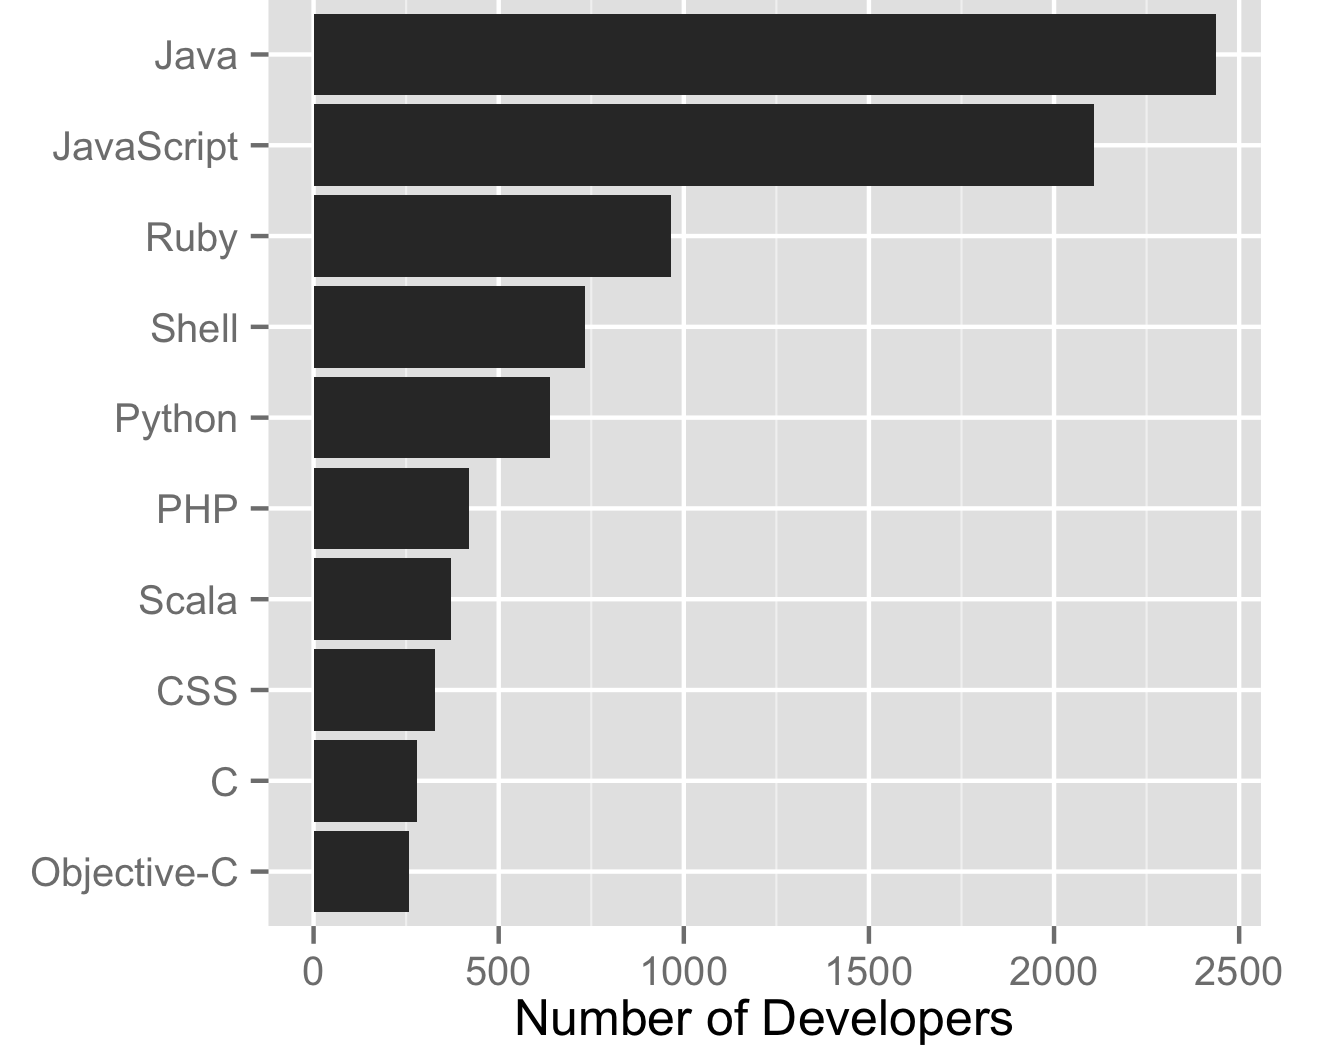
\includegraphics[width=0.6\textwidth]{../aosd_2014/analysis/result/languages.png}
\caption{Most popular languages among Groovy developers}
\label{fig:other_languages} 
\end{figure}

% \begin{figure}[ht]
% \centering 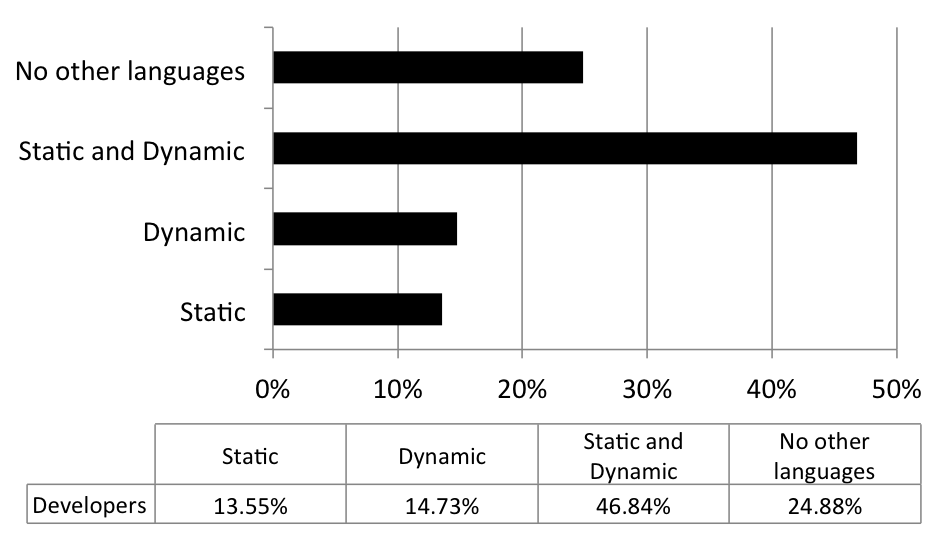
\includegraphics[width=0.7\textwidth]{typeSystem_background}
% \caption{Type System of other languages used by programmers}
% \label{fig:typeSystem_background} 
% \end{figure}


%ANALYZER
\section{Static Code Analyzer\label{analyzer}}
In order to understand in which situations programmers use types, we developed a static code analyzer based on the Groovy metaprogramming library.
This analyzer is capable of retrieving the declaration information of parameters and returns of methods, parameters of constructors, fields and local variables.
In addition, the analyzer can tell if a declaration is part of a test class or a script and what is its visibility.

A relevant decision we made was not to compile projects, which would require all dependencies to be resolved.
This is not feasible given the size of our dataset.
Instead, we generated the AST for each file using the \emph{CONVERSION} phase of the Groovy compiler.
At this phase, the compiler has not tried to resolve any dependencies yet, but it is capable of generating an AST with enough information to determine whether a declaration is typed or not.
This makes it possible to analyze each Groovy file separately without having to compile the whole project.
The downside of this approach is that we cannot analyze Groovy code in conjunction with its dependencies. 
For example, it is not possible to determine whether programmers tend to type code that interacts with other typed modules since we have not resolved any dependencies on these modules.
However, our choice was fundamental in order to execute a study with such an extensive dataset.
% Nevertheless, as shown in the next section, we were still able to obtain detailed and relevant results.











%
% RESULTS
%
\chapter{Results\label{results}}
This section presents the data obtained from our analysis.
Section \ref{sec:results-overall} shows the overall result.
The usage of types according to the kind and visibility of declarations are presented in Sections \ref{sec:results-type} and \ref{sec:results-visibility}.
Section \ref{sec:results-tests} shows how types are used in test and functional classes while Section \ref{sec:results-scripts} compares the usage of types in script and class files.
We study the influence of programmers' background in Section \ref{sec:results-background} and how types are used according to age, size and number of commits of projects in Section \ref{sec:results-maturity}.
Finally, we analyze the usage of types according to frequency of changes of files in Section \ref{sec:results-changes}.
In this section we focus on the presentation and on the statistical treatment of the obtained results.
Their interpretation is left to Chapter \ref{discussion}.

\section{Overall Result\label{sec:results-overall}}

This section presents an overview of the results.
Figure \ref{fig:all_histogram_all} shows a histogram and the descriptive statistics for the relative usage of types in declarations of projects.
This value can vary from 0 (a project does not declare any types) to 1 (all declarations of a project are typed). 
All declarations are considered without making any distinction among them.

\begin{figure}[h]
\centering 
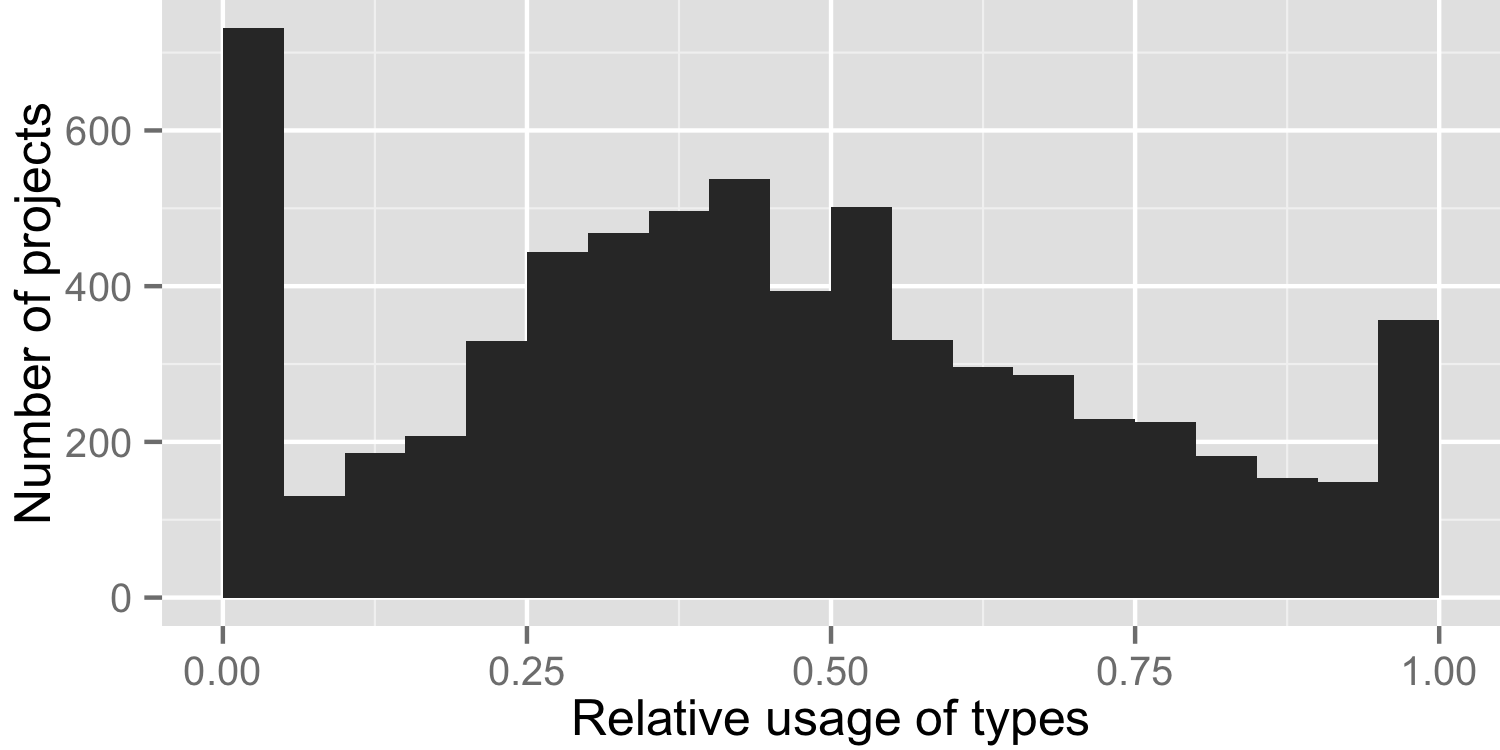
\includegraphics[width=0.7\textwidth]{../aosd_2014/analysis/result/all/histograms/5_all_types.png} 

\vspace{0.3cm}

\begin{tabular}{|c|c|c|cccc|}
\hline
{}		&  {}		&  {}			&  \multicolumn{4}{c|}{Quartiles}				\\
n		& mean	& std. dev.	& 1\ts{st}	& 2\ts{nd}	& 3\ts{rd}	& 4\ts{th}		\\
\hline
\hline
6638 	& 0.45	& 0.28		& 0.25	& 0.42		& 0.64	& 1.00		\\
\hline
\end{tabular}


\caption{Usage of types in all declarations of all projects}
\label{fig:all_histogram_all} 
\end{figure}

Note that there is a significant number of projects for which the relative usage of types is either approximately 0 or 1.
These are mostly small projects.
About 95\% of them have less than 1000 lines of code and 22\% of them have less than 100 lines of code.
In such projects, it is easier to be consistent on the typing strategy since there are just a few declarations.
We initially considered not including these projects in the rest of our analysis since they could not represent well the entire population of Groovy projects.
However, doing so did not alter the results significantly and we decided to include all projects in our analysis regardless of their size.
In the rest of this section, this data will be presented in more detail so we can understand which factors lead programmers to use types or not.


% TYPE
\section{Kind of Declaration\label{sec:results-type}}
This section investigates whether programmers use types differently depending on the kind of the declaration.
For each project, we measured the relative usage of types in fields, constructor parameters, method returns, method parameters and local variables.
These results are displayed in box plots in Figure \ref{fig:all_boxplot_type} along with the corresponding descriptive statistics.
Note that the size of each sample, \emph{n}, is different since not all projects have all types of declarations. 
For instance, there are only 1670 out of 6638 projects that declare constructor parameters.
On the other hand, 6000 projects have declarations of fields.

\begin{figure}[h]
\centering 
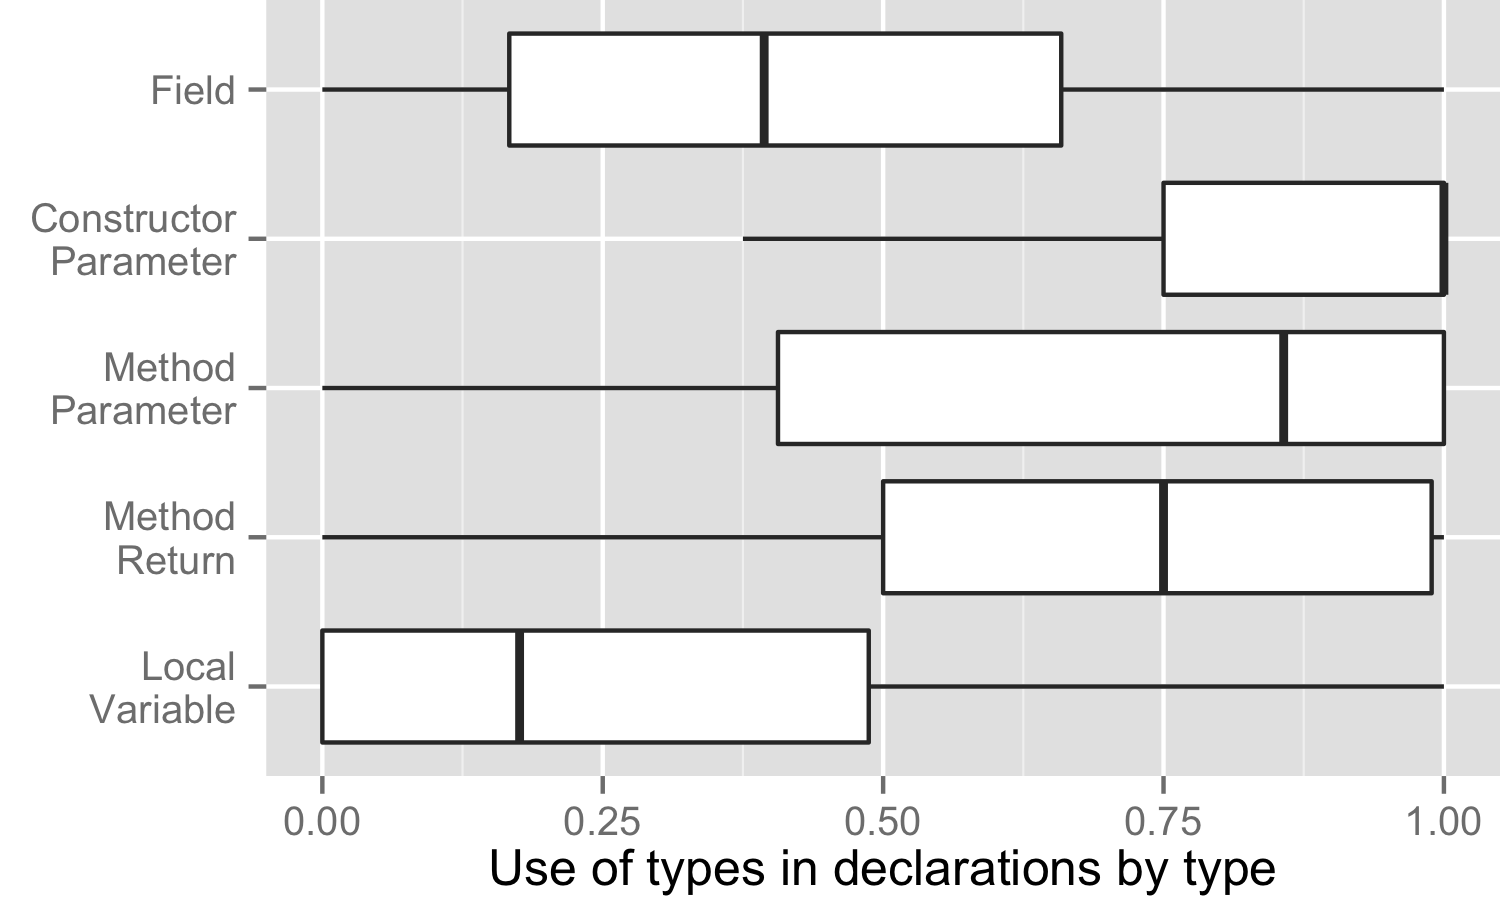
\includegraphics[width=0.7\textwidth]{../aosd_2014/analysis/result/all/boxplots/6_declarations_by_type.png} 
\vspace{0.3cm}

\renewcommand{\arraystretch}{1.2}

\begin{tabular}{|c|c|c|c|c|}
\hline
Declaration Type		& n		& mean	& median		& std. dev.	\\
\hline
\hline
Field					& 6000	& 0.43	& 0.39		& 0.33		\\ \hline
Constructor Parameter	& 1670	& 0.80	& 1.00		& 0.35		\\ \hline
Method Parameter		& 4867	& 0.67	& 0.86		& 0.36		\\ \hline
Method Return			& 5881	& 0.68	& 0.75		& 0.31		\\ \hline
Local Variable			& 5845	& 0.29	& 0.18		& 0.32		\\ \hline
\end{tabular}

\caption{Usage of types in all declarations by type of declaration}
\label{fig:all_boxplot_type} 
\end{figure}



The results presented in Figure \ref{fig:all_boxplot_type} suggest that programmers use types differently depending on the type of a declaration.
Local variables, for example, are typed less often.
Half of the projects have only 18\% or less of their local variables typed.
Conversely, methods and constructors are typed in most cases.
Note that the median for constructor parameters is equal to 1.00, which means that at least half of the projects with constructor parameters type all declarations of this kind.
Since local variables are never part of a module interface, these results suggest a positive answer for Question Q1, i.e, declarations that compose module interfaces are typed more often than other declarations.

The box plot graph and the descriptive statistics are not enough to determine whether the difference in the usage of types in any two kinds of declaration is significant.
In order to do that, a significance test should be applied. 
We start by defining a hypothesis below, which can then be rejected or accepted by the test.

% Rewrite the hypothesis for ANOVA
\begin{description}
\item[H0] There is no difference in how programmers type different kinds of declarations
\item[H1] Programmers type their declarations differently depending on the kind of the declaration
\end{description}

The appropriate significance test should be chosen carefully.
It needs to compare multiple treatments, which represent the 5 distinct kinds of declaration.
We first considered applying repeated \emph{t-tests} or \emph{Mann-Whitney U-tests} (\cite{Wohlin2012}) in order to compare every two kinds of declaration, i.e, fields vs. local variables, fields vs method returns, etc.
However, applying repeated tests over the same sample increases the probability of getting Type-I errors (rejecting the null hypothesis when it actually should be accepted).

A valid alternative for our scenario is to use One-Way Between Groups ANOVA, which compares all means simultaneously and maintains the Type-I error probability at the designated level (\cite{Wohlin2012}).
ANOVA computes a \emph{p} value which indicates whether at least two treatments are significantly different from each other.
The smaller the value of \emph{p}, the "more significant" is the difference and, consequently, the stronger the rejection of the null hypothesis.

Given the level of significance, $\alpha$, we can reject the null hypothesis if $p < \alpha$.
Typically, $\alpha=0.05$ or $\alpha=0.01$ are used, but in this study  we decided to use a very small value for this purpose, $\alpha=0.001$.
This value might seem too small at first, which would require the difference between two treatments to be unnecessarily high in order to be considered significant.
However, since we are analyzing such a large dataset, this value of $\alpha$ seems reasonable (\cite{labovitz68}).
For the treatments described in Figure \ref{fig:all_boxplot_type} the \emph{p} value reported by ANOVA is 0. 
This allows us to strongly reject the null hypothesis, even though we are using such an extreme value for $\alpha$, and state that at least two treatments are different from each other.

% In addition to the \emph{p} value, it is also possible to determine the effect size, $\eta^2$, which is a measure of how much an independent variable has affected % the dependent variable.
% In other words, we can use the effect size to determine the extent to which the kind of declaration has influenced programmers on their choice whether to type or not % their declarations.
% We follow the guidelines proposed by Cohen's in order to determine how big is the value of $\eta^2$ \cite{Cohen88}.
% These guidelines suggest that values inferior to 0.01 represent a small effect, values up to 0.0589 indicate medium effects and 0.138 or more represents large effects% .
% In our analysis, we obtained $\eta^2=0.22$, which indicates a very large effect size.
% This result implies that the usage of types in declarations is largely influenced by the kind of declaration.

The results above show a very clear influence of the kind of variable over the usage of types.
However, it is also desirable to know which kinds of variables are different from each other and how different they are.
For this purpose, we apply the Tukey Honestly Significant Differences (\cite{kirk1995}), or Tukey HSD, test in conjunction with ANOVA.
This method calculates, for every two treatments, a \emph{p} value indicating whether they are significantly different.
It also reports a confidence interval for the difference between the means of these two treatments.
The results of the Tukey Honest Significant Differences are displayed in Table \ref{tab:all_utest_type}.
Confidence intervals were calculated with a confidence of 0.999 ($1-\alpha$).


% Use a super small significance level
% Labovitz, Sanford. "Criteria for selecting a significance level: A note on the sacredness of. 05." The American Sociologist 3.3 (1968): 220-222.

% ETA 0.2797227
\begin{table}[ht]

\centering{}%
\renewcommand{\arraystretch}{1.2}

\caption{Tukey Honest Significant Differences Test results for the comparison between the usage of types by kind of declaration}
\begin{tabular}{|c|c|c|c|}
\hline 
                & {}          & p         & Difference \\
\hline
\hline
Local Variable & Contructor Parameter & 0      & (-0.55, -0.47) \\ \hline
Field & Contructor Parameter & 0      & (-0.41, -0.34) \\ \hline
Method Parameter & Contructor Parameter & 0      & (-0.17, -0.10) \\ \hline
Method Return & Contructor Parameter & 0      & (-0.16, -0.09) \\ \hline
Local Variable & Field & 0      & (-0.16, -0.11) \\ \hline
Method Return & Field & 0      & ( 0.22,  0.26) \\ \hline
Method Parameter & Field & 0      & ( 0.22,  0.27) \\ \hline
Method Parameter& Local Variable & 0      & ( 0.35,  0.40) \\ \hline
Method Return & Local Variable & 0      & ( 0.36,  0.41) \\ \hline
Method Return & Method Parameter& 0.95 & (-0.02,  0.03) \\ \hline
\end{tabular}
\label{tab:all_utest_type}
\end{table}




%The confidence interval shows what is the difference of means between the declaration types shown in the first and second columns.
%For example, the confidence interval of the first row indicates with a confidence level of 99\% that the difference between the medians of fields %and constructor parameters is between $-0.50$ and $-0.44$.
The table above shows that there are only two kinds of declaration for which there is no significant difference, parameters and returns of methods.
This result is reasonable.
Since returns and parameters of methods are declared together as part of a method signature, programmers probably use the same typing strategy in both declarations.
All other declaration types can be considered significantly different from each other.
In particular, note that these results clearly show that local variables and constructor parameters are the least and most typed declarations respectively.
Another interesting insight provided by these results is that parameters of methods and parameters of constructors are typed differently.
Although these are essentially the same kind of declaration in Groovy, they seem to be perceived differently by programmers when it comes to typing.




% VISIBILITY
\section{Declaration Visibility\label{sec:results-visibility}}

This section presents an analysis about how programmers use types according to the visibility of a declaration.
We follow the same approach as in the previous section.
Figure \ref{fig:all_boxplot_visibility_all} shows the box plots for the usage of types per declaration visibility along with the descriptive statistics.
The ANOVA test reported a \emph{p} value equal to 0 for these treatments, allowing us to strongly reject the null hypothesis.
% The obtained effect size was again very large, $\eta^2=0.28$, implying that there is a very large influence of the visibility of a declaration over the value of the relative usage of types.
Finally, the results of the Tukey HSD Test are reported in Table \ref{tab:all_utest_visibility}.
These results show that all treatments are different from each other since all \emph{p} values are equal to 0.


\begin{figure}[h!]
\centering 
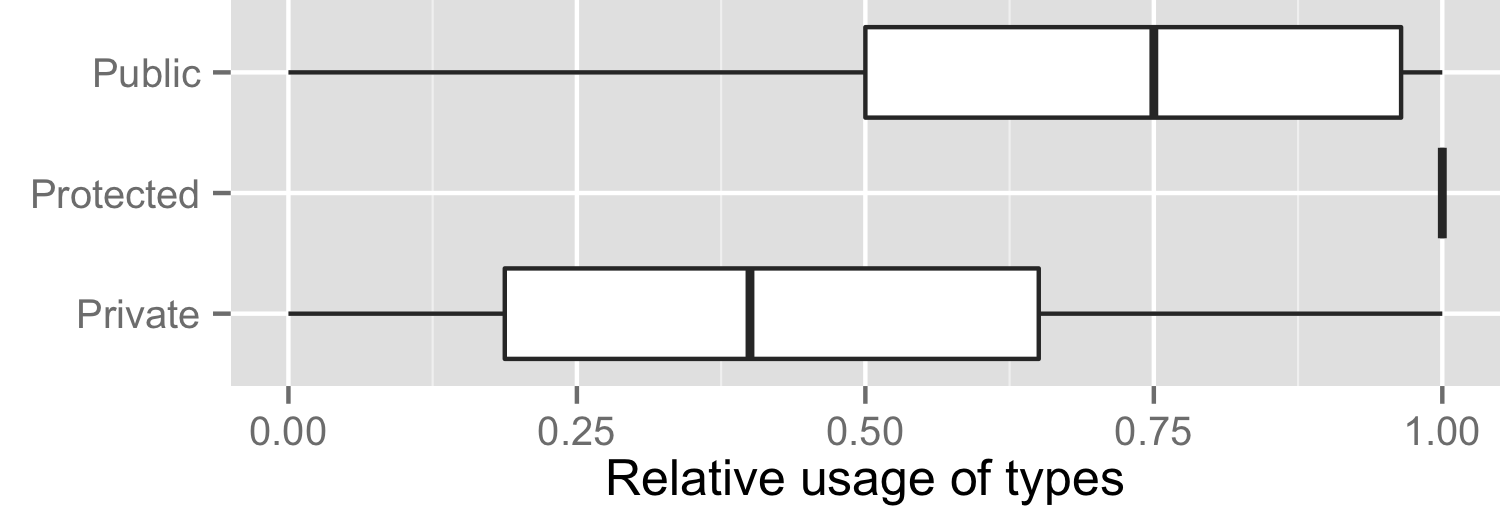
\includegraphics[width=0.7\textwidth]{../aosd_2014/analysis/result/all/boxplots/23_declarations_by_visibility.png} 


\vspace{0.3cm}

\renewcommand{\arraystretch}{1.2}

\begin{tabular}{|c|c|c|c|c|}
\hline
Declaration Visibility	& n		& mean	& median	& std. dev.	\\
\hline
\hline
Public    				& 5852	& 0.69	& 0.75		& 0.29		\\ \hline
Protected 				& 2387	& 0.93	& 1.00		& 0.19		\\ \hline
Private   				& 6023	& 0.43	& 0.40		& 0.32		\\ \hline
\end{tabular}
\caption{Usage of types in all declarations by type of declaration}
\label{fig:all_boxplot_visibility_all} 
\end{figure}

\begin{table}[h]

\centering{}%
\renewcommand{\arraystretch}{1.2}

\caption{Tukey Honest Significant Differences Test results for the comparison between the usage of types by visibility of declaration}
\begin{tabular}{|c|c|c|c|}
\hline 
                & {}    & p   & Difference  \\
\hline
\hline
Protected & Private & 0 & ( 0.47,  0.52) \\ \hline
Public & Private & 0 & ( 0.24,  0.28) \\ \hline
Public & Protected & 0 & (-0.27, -0.22) \\ \hline
\end{tabular}
\label{tab:all_utest_visibility}
\end{table}

Protected declarations are those typed most often.
Note how skewed is the distribution for these elements in Figure \ref{fig:all_boxplot_visibility_all}.
Almost all 2387 projects which use protected visibility in their declarations have all of their protected fields, methods and constructors typed.
The confidence intervals reported by the Tukey HSD test show very large differences between these declarations and those with either private or public visibility.
Although public declarations are not typed as much, they are also typed very often.
At least half of the projects type 75\% or more of their public declarations.
Conversely, private declarations are those with the smallest relative use of types.
These results again suggest a positive answer for Question Q1, which hypothesizes that declarations that are part of a module interface definition are typed more frequently.


% BREAKING VISIBILITY BY DECLARATION TYPE
% Figures \ref{fig:all_boxplot_visibility_methodReturn}-\ref{fig:all_boxplot_visibility_field} detail these results by declaration type.
% \begin{figure}[h]
% \centering 
% 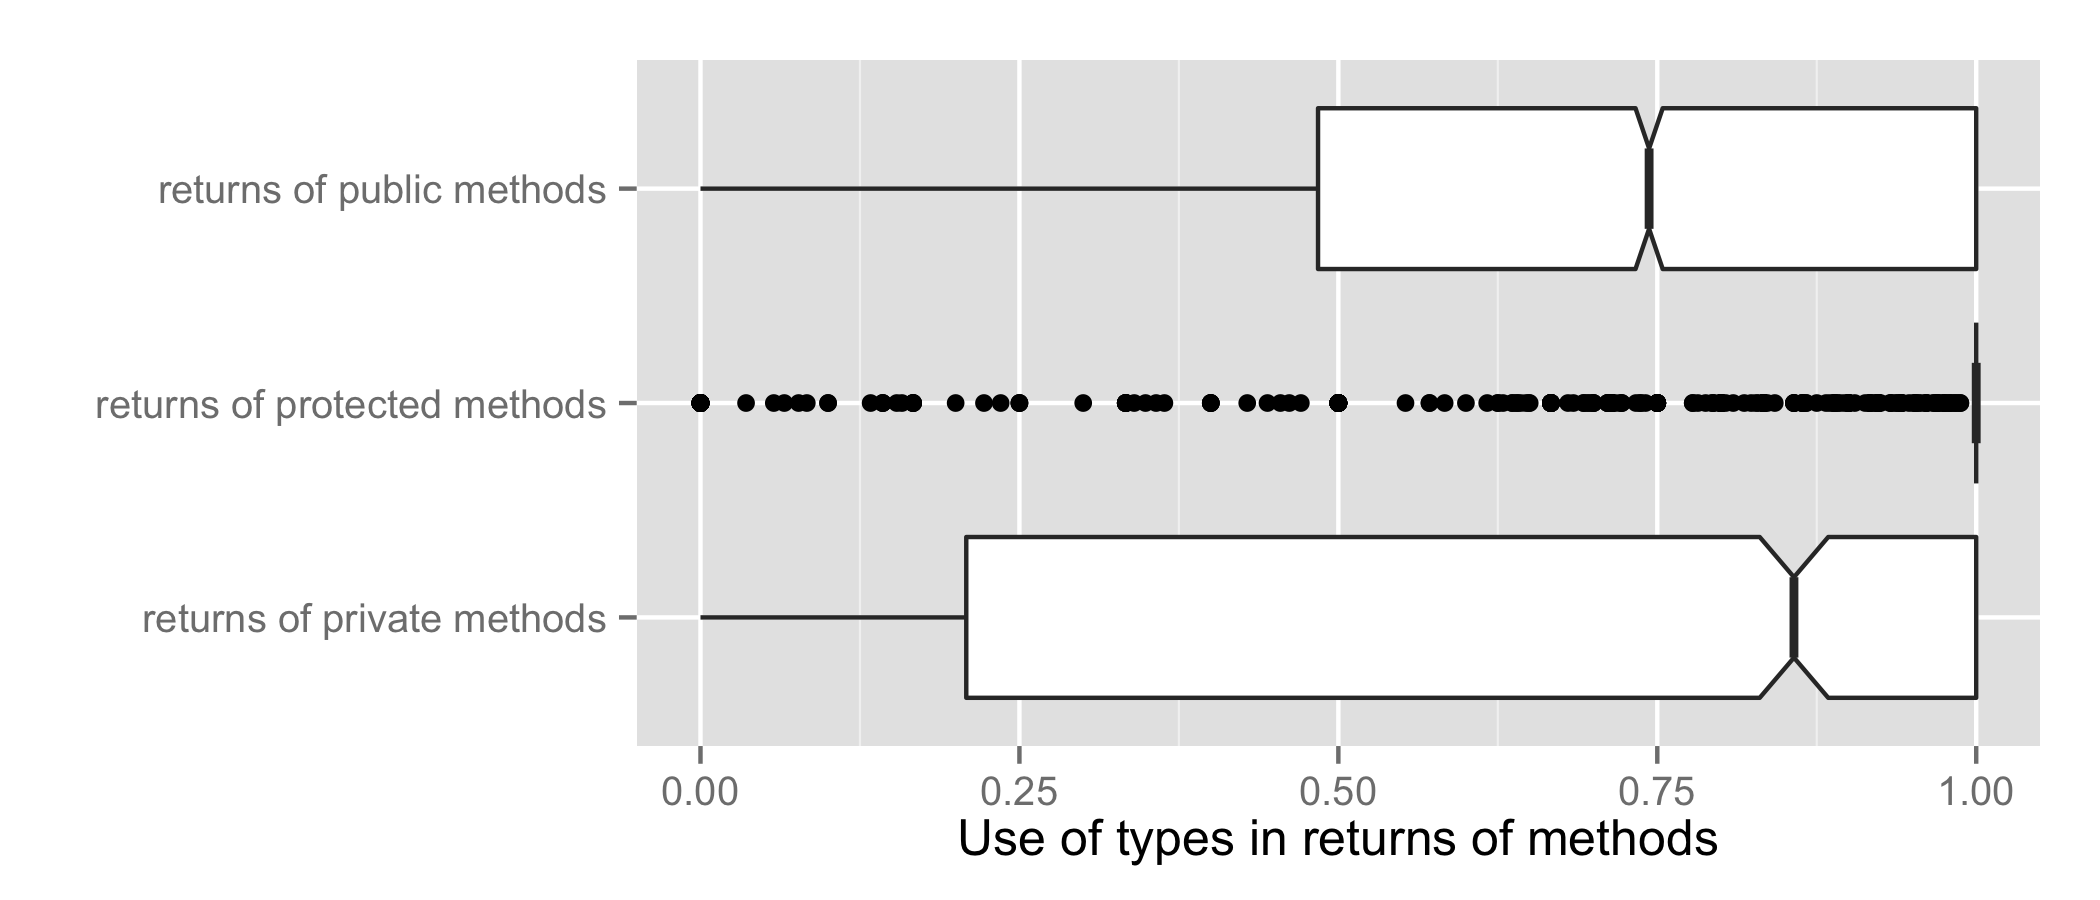
\includegraphics[width=0.7\textwidth]{../aosd_2014/analysis/result/all/boxplots/11_returns_of_methods.png} 
% \caption{Usage of types in declarations of returns of methods by visibility}
% \label{fig:all_boxplot_visibility_methodReturn} 
% \end{figure}
% 
% \begin{figure}[h]
% \centering 
% 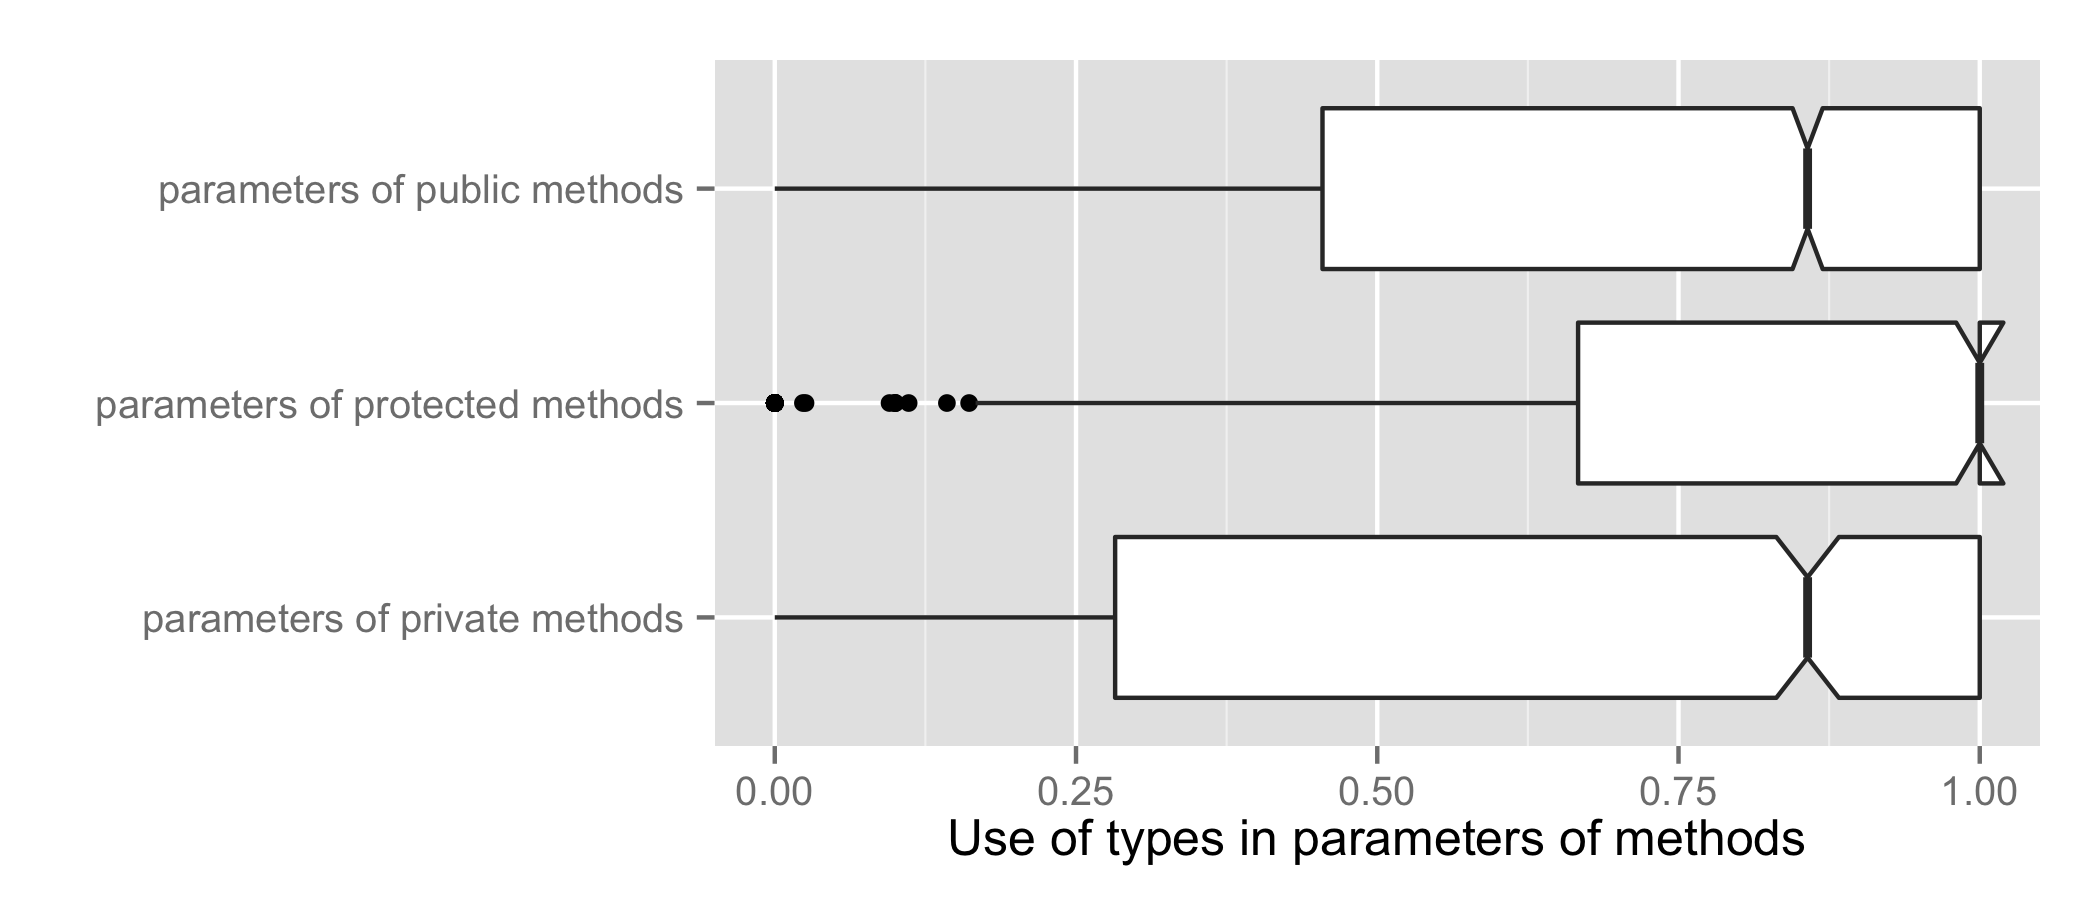
\includegraphics[width=0.7\textwidth]{../aosd_2014/analysis/result/all/boxplots/14_parameters_of_methods.png} 
% \caption{Usage of types in declarations of parameters of methods by visibility}
% \label{fig:all_boxplot_visibility_methodParameter} 
% \end{figure}
% 
% \begin{figure}[h]
% \centering 
% 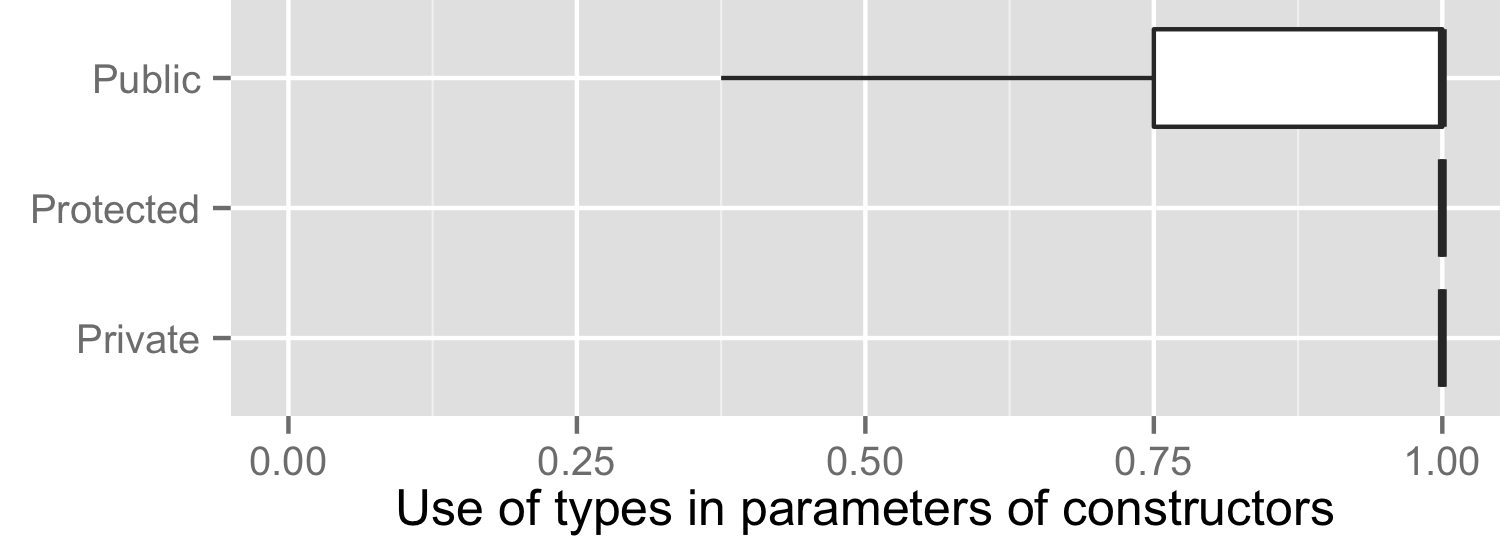
\includegraphics[width=0.7\textwidth]{../aosd_2014/analysis/result/all/boxplots/17_parameters_of_constructors.png} 
% \caption{Usage of types in declarations of constructor parameters by visibility}
% \label{fig:all_boxplot_visibility_constructorParameter} 
% \end{figure}
% 
% \begin{figure}[h]
% \centering 
% 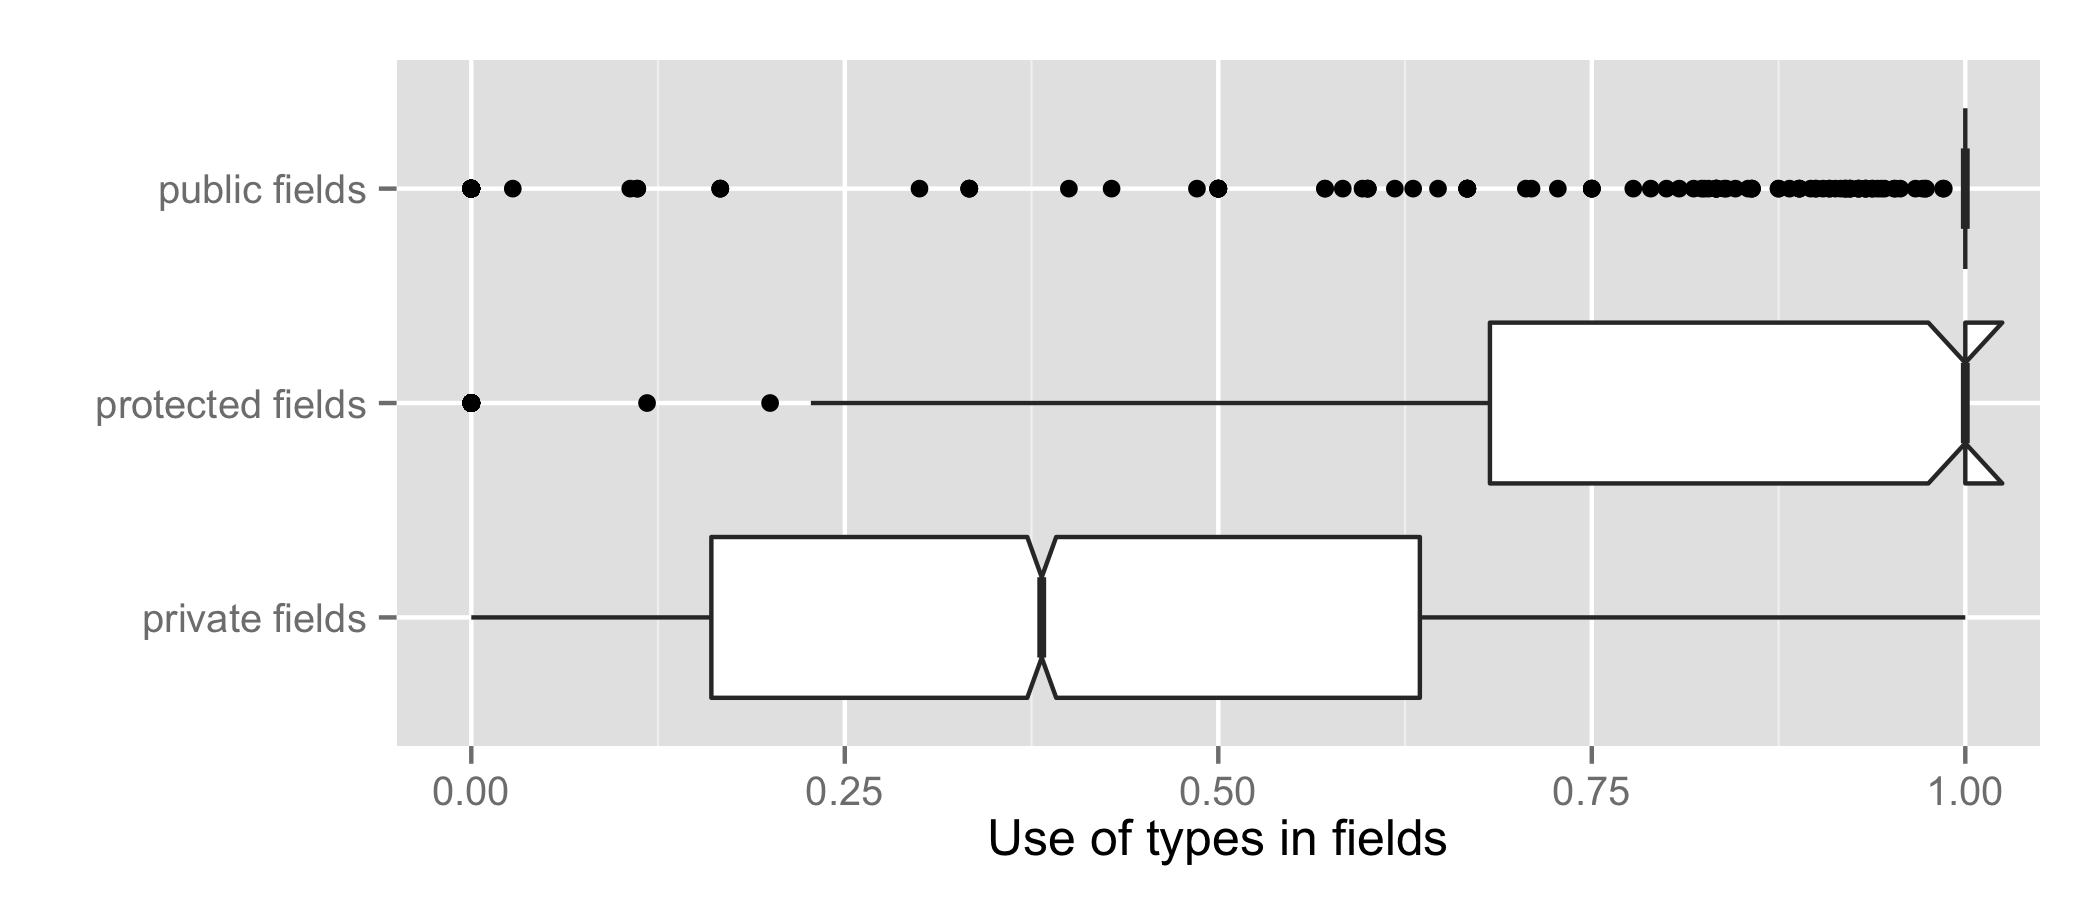
\includegraphics[width=0.7\textwidth]{../aosd_2014/analysis/result/all/boxplots/20_fields.png} 
% \caption{Usage of types in declarations of fields by visibility}
% \label{fig:all_boxplot_visibility_field} 
% \end{figure}





% TESTS
\section{Test Classes and Main Classes\label{sec:results-tests}}
We now analyze the use of types in test classes in comparison to main classes.
We used a simple heuristic to determine the kind of the class.
In Groovy, like in Java, it is common to organize test classes and main classes in different source folders.
The convention adopted by build tools popular among Groovy programmers, such as Gradle and Maven, assumes that test classes and main classes are in the \emph{src/test/groovy} and \emph{src/main/groovy} directories respectively.
Based on these conventions, we assume that all classes inside a \emph{test} directory, but not in a \emph{main} directory, are test classes.

For every project, we measured the usage of types in test classes and main classes.
Script files are not considered in this analysis.
We found test classes in 4350 of the 6638 projects in our dataset.
Results are displayed in Figure \ref{fig:test_boxplot_type} and show the relative usage of types by declaration type.
White and gray box plots correspond to test classes and main classes respectively.

In order to compare the usage of types in test and main classes, we use a slightly different approach.
In this analysis, there are two independent variables, the kind of declaration and the kind of class.
Thus, we are required to use Factorial ANOVA (\cite{Wohlin2012}), which is the generalization of the One Way ANOVA for multiple factors.
Multiple values of \emph{p} are calculated by this test, each one corresponding to the comparison of treatments according to one of the factors.
We report the \emph{p} value corresponding to the factor representing the kind of class.
We also apply the Tukey HSD test, for which results are displayed in Table \ref{tab:test_utest_type}.
This time we want to show what is the difference of the relative usage of types between the same kinds of declaration, but in different kinds of classes.
For example, the third row of Table \ref{tab:test_utest_type} shows that there is a significant difference in how programmers type local variables in main and test classes.
The overall difference between the relative usage of types in main classes and test classes falls in the $(0.05, 0.11)$ interval.

The ANOVA test reported once again a \emph{p} value equal to 0, implying that the usage of types is different in test and main classes.
Figure \ref{fig:test_boxplot_type} and Table \ref{tab:test_utest_type} show that this difference is significant for all kinds of declarations, except for constructor parameters.
While local variables in main classes are not typed very often, they are typed even less in test classes.
At least half of the projects type none of the declarations of this kind in test classes.
The difference in declarations of parameters of methods is even more evident since they are often typed in main classes, but almost never typed in test classes.
The confidence interval reported by the Tukey HSD Test in this case is $(-0.36, -0.44)$.
The large width of the box plots for fields and method parameters is noteworthy.
This indicates that many projects type either almost all or none of these declarations.
\begin{figure}[h]
\centering 
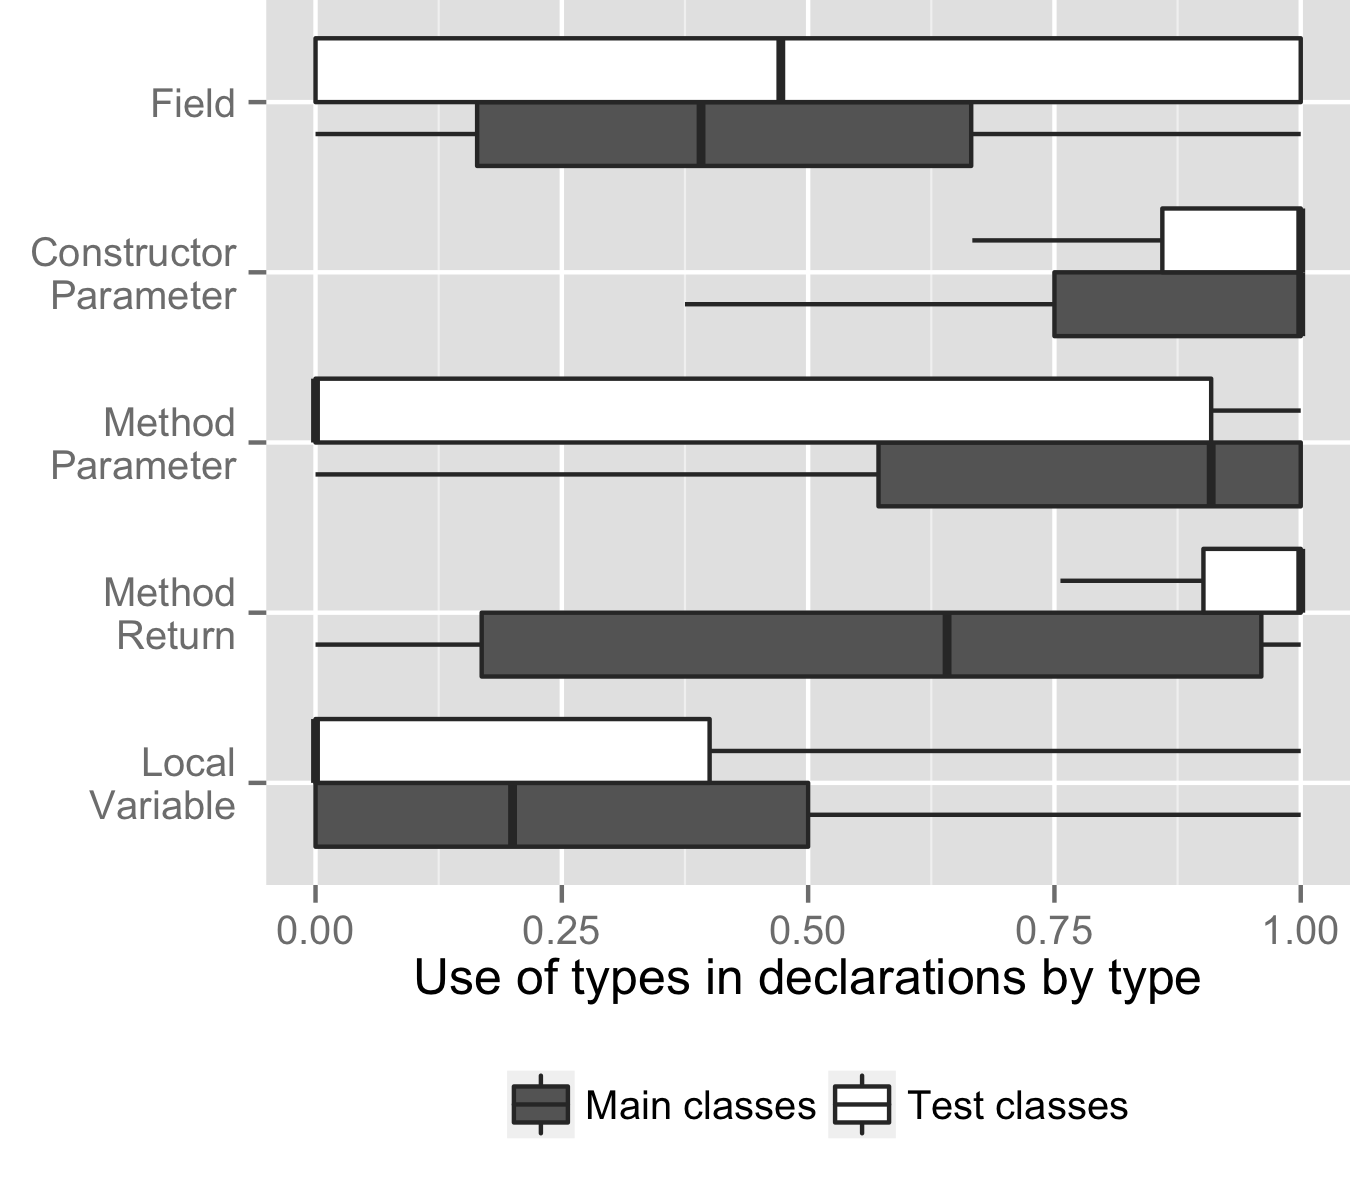
\includegraphics[width=0.7\textwidth]{../aosd_2014/analysis/result/test/comparison/boxplots/6_declarations_by_type.png} 
\vspace{0.1cm}
\renewcommand{\arraystretch}{1.2}


\begin{tabular}{|c|c|c|c|c|c|}
\hline
\cell{Declaration Type}	& \cell{Class Type}& n		& mean		& median	& \cell{std. dev.}\\
\hline
\hline
\multirow{2}{*}{Field}	& Test			& 1769	& 0.48 		& 0.47	& 0.43 \\ 
                		& Main			& 5857	& 0.43 		& 0.39	& 0.33 \\
\hline                
Constructor 			& Test			&  124	& 0.77 		& 1.00	& 0.41 \\                
Parameter				& Main			& 1623	& 0.80 		& 1.00	& 0.34 \\                
\hline
Method      			& Test			& 1524	& 0.34 		& 0.00	& 0.43 \\                
Parameter				& Main			& 4593	& 0.71 		& 0.91	& 0.35 \\                
\hline
Method      			& Test			& 4334	& 0.85 		& 1.00	& 0.31 \\                
Return		         	& Main			& 5299	& 0.54 		& 0.60	& 0.39 \\                
\hline
Local					& Test			& 2842	& 0.23 		& 0.00	& 0.35 \\                
Variable	        	& Main			& 5548	& 0.30 		& 0.19	& 0.32 \\                
\hline
\end{tabular}

\caption{Usage of types by declaration type in test classes and main classes}
\label{fig:test_boxplot_type} 
\end{figure}

\FloatBarrier




% ETA=0.072
\begin{table}[h!]
\centering{}%

\caption{Tukey Honest Significant Differences Test results for the comparison between the usage of types by main and test classes}
\begin{tabular}{|c|c|c|}
\hline 
Declaration Type    & p & Difference \\
\hline 
\hline 
Constructor Parameter &  0.98     & (-0.08,  0.16) \\ \hline
Field &  0          & (-0.08, -0.02)  \\ \hline
Local Variable &  0          & ( 0.05,  0.11) \\ \hline
Method Parameter &  0          & ( 0.36,  0.44) \\ \hline
Method Return &  0          & (-0.31, -0.26) \\ \hline
\end{tabular}
\label{tab:test_utest_type}
\end{table}




Curiously, method returns are significantly more typed in test classes.
The difference reported by the confidence interval in Table \ref{tab:test_utest_type} for this case is (-0.31, -0.26).
At least half of the projects type all of their method returns in test classes.
Although counterintuitive, this result can be easily explained.
Automated testing frameworks usually enforce a certain method signature for test methods.
JUnit, for example, which is used in 2525 of the 4350 projects with test classes, requires test methods to be typed as \emph{void}.
Other popular test frameworks, such as TestNG, have similar requirements.
This implies that, in this case, developers type their methods not because they want to, but because they have to.





% SCRIPTS
\section{Script Files and Class Files\label{sec:results-scripts}}
In Groovy, programmers can write code in the form of scripts, not requiring the definition of classes for simple tasks.
This section investigates how programmers type their code in such scripts.
Similar to what was done in the previous section, we measured the usage of types in script and class files in all projects and compared the obtained data.
We do not consider test classes in this analysis.
Determining whether a file corresponds to a script or a class is fairly simple since, in Groovy, scripts are compiled into a class extending \emph{groovy.lang.Script}.

Figure \ref{fig:script_boxplot_type} shows the distribution of the relative usage of types in class and script files.
Note that constructors and fields are not considered since there is no way to declare those elements in scripts.
Also, we do not present an analysis of declarations grouped by visibility since, although allowed, defining the visibility of a declaration inside a script does not make much sense.



The execution of the ANOVA test reported a \emph{p} value equal to 0, revealing that the declarations are typed significantly different in script files.
Table \ref{tab:script_utest_all} displays the results for the Tukey HSD test, which provide detailed results by the kind of declaration.
There is no significant difference on the usage of types in local variables.
On the other hand, declarations of parameters or returns of methods are typed much less frequently in scripts.
Note however that the value for the last quartile of these declarations is very high, superior to 0.8.
This indicates that, although most projects prefer not to use types in method returns, there are a few projects that consistently type most of them.

\begin{figure}[h]
\centering 
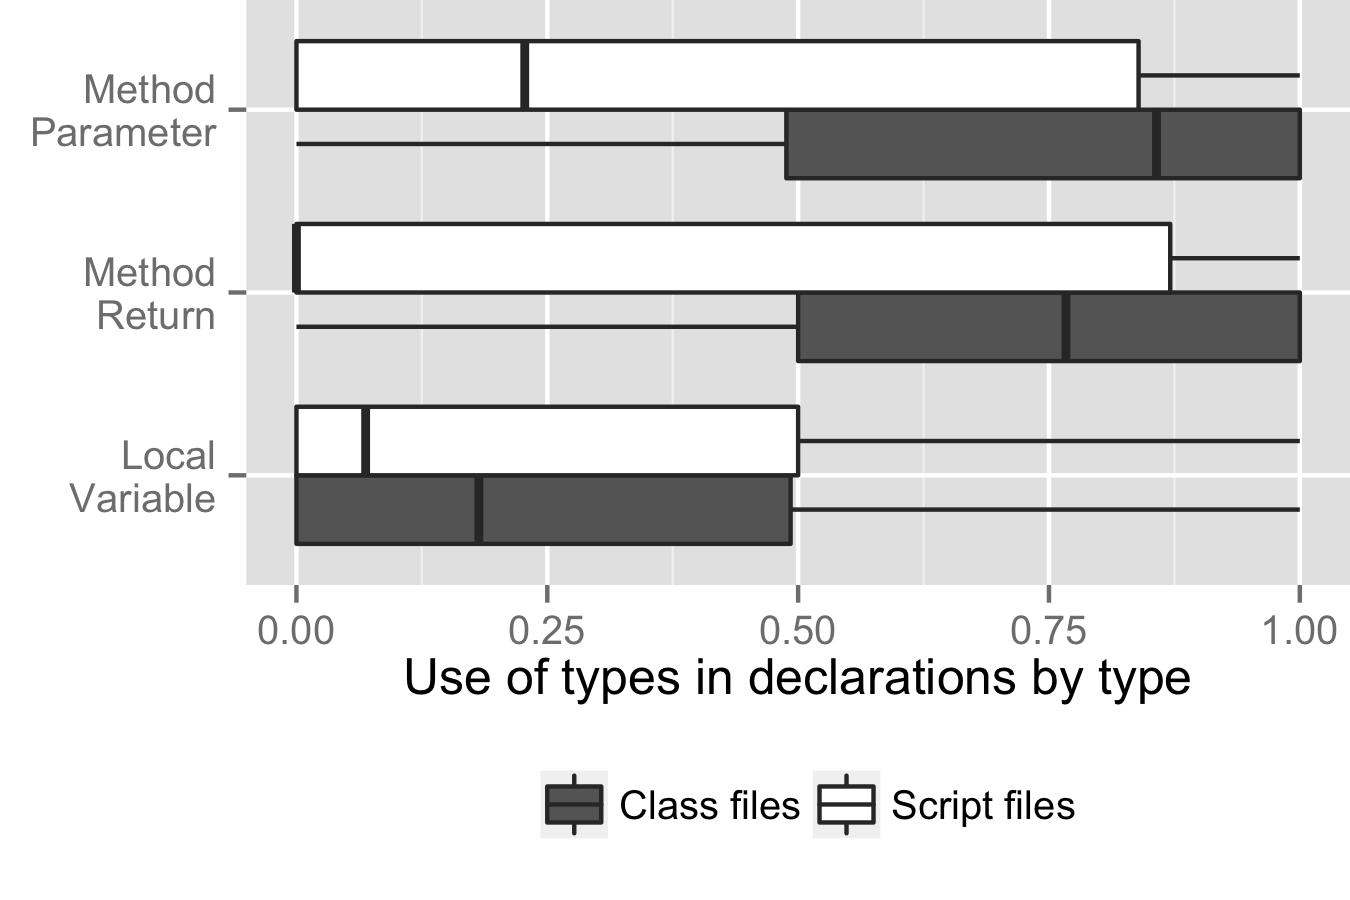
\includegraphics[width=0.7\textwidth]{../aosd_2014/analysis/result/script/comparison/boxplots/6_declarations_by_type.png} 
\vspace{0.1cm}
\renewcommand{\arraystretch}{1.2}


\begin{tabular}{|c|c|c|c|c|c|}
\hline
\cell{Declaration Type}&\cell{File Type}	& n		& mean		& median	& \cell{std. dev.}\\
\hline
\hline	
Method					& Script			& 504 	& 0.40	& 0.23	& 0.42	 \\                
Parameter					& Class				& 4647	& 0.69	& 0.86	& 0.35	 \\                \hline	
Method					& Script			& 583 	& 0.34	& 0.00	& 0.43	 \\                
Return					& Class				& 5662	& 0.70	& 0.77	& 0.30	 \\                \hline	
Local					& Script			& 1775	& 0.28	& 0.07	& 0.37	 \\                
Variable	 				& Class				& 5246	& 0.30	& 0.18	& 0.32	 \\                
\hline
\end{tabular}
\caption{Usage of types by declaration type in script files and class files}
\label{fig:script_boxplot_type} 
\end{figure}

\FloatBarrier
% ETA=0.067
\begin{table}[ht]
\centering{}%

\caption{Tukey Honest Significant Differences Test results for the comparison between the usage of types in script files and class files}
\begin{tabular}{|c|c|c|}
\hline 
Declaration Type & p & Difference \\
\hline 
\hline 
Local Variable   & 0.39 & (-0.01, 0.04) \\ \hline
Method Parameter & 0    & ( 0.24, 0.35) \\ \hline
Method Return    & 0    & ( 0.30, 0.40) \\ \hline
\end{tabular}
\label{tab:script_utest_all}
\end{table}

Along with the results of the analysis of test classes, the results presented in this section show that the answer for Question Q2 is positive.
There are large differences in how programmers type scripts and classes.
Although it is not clear from our analysis what is the reason for such phenomena, we discuss some hypotheses in Chapter \ref{discussion}.




% PROGRAMMERS BACKGROUND
\section{Programmers' Background\label{sec:results-background}}
In this section, we analyze how programmers use types in their declarations according to their backgrounds.
Projects are distributed in three groups based on the type system of the languages their developers have used on GitHub.
The first group comprises those projects of programmers who developed only in statically typed languages, such as Java or C\#.
The projects of those who developed only in dynamically typed languages, such as Ruby or JavaScript, comprise the second group.
Finally, the third group is formed by the projects of those programmers with both dynamically and statically typed languages in their portfolio.
We refer to these three groups by the names \emph{Static Only}, \emph{Dynamic Only} and \emph{Static and Dynamic} respectively.

Figures \ref{fig:background_boxplot_type} and \ref{fig:background_boxplot_visibility}  show results by declaration type and visibility respectively.
The \emph{p} value reported by the ANOVA test is equal to 0, implying that there is a significant difference in how programmers with different backgrounds type their declarations.
The results of the Tukey HSD test are reported in Tables \ref{tab:background_utest_type} and \ref{tab:backgorund_utest_visibility}.
These tables are divided in three parts, each one corresponding to the comparison between the data of two of the three groups.

There are significant differences in the usage of types between all groups.
These differences, however, are not as clear as those found in the previous anlayses.
Let's start with the comparison between projects in the \emph{Static and Dynamic} and the \emph{Dynamic Only} groups.
There are significant differences only in private declarations and declarations of fields.
Still, these differences are not very large, $(0.01,0.08)$ for fields and $(0.02,0.09)$ for private declarations.
All in all, these two groups present very similar behavior when typing their declarations, apart from those two exceptions.
                

The comparison between the \emph{Static} and the other groups shows more clear differences.
Most of the \emph{p} values reported by the Tukey HSD test are equal to 0.
However, constructor parameters and protected declarations never present significant differences.
This indicates a strong influence of these types of declarations over the programmers' behavior.
There are two other cases that do not present significant differences, method returns and public declarations, both in the comparisons between programmers of the \emph{Dynamic} and \emph{Static} groups.
It is important to say though that the \emph{p} value reported in these two cases is relatively small, 0.01.
These differences are considered not significant only because we are using a very strict confidence level, but would be considered significantly different under a confidence level of 0.05.

\begin{figure}[ht!]
\centering 
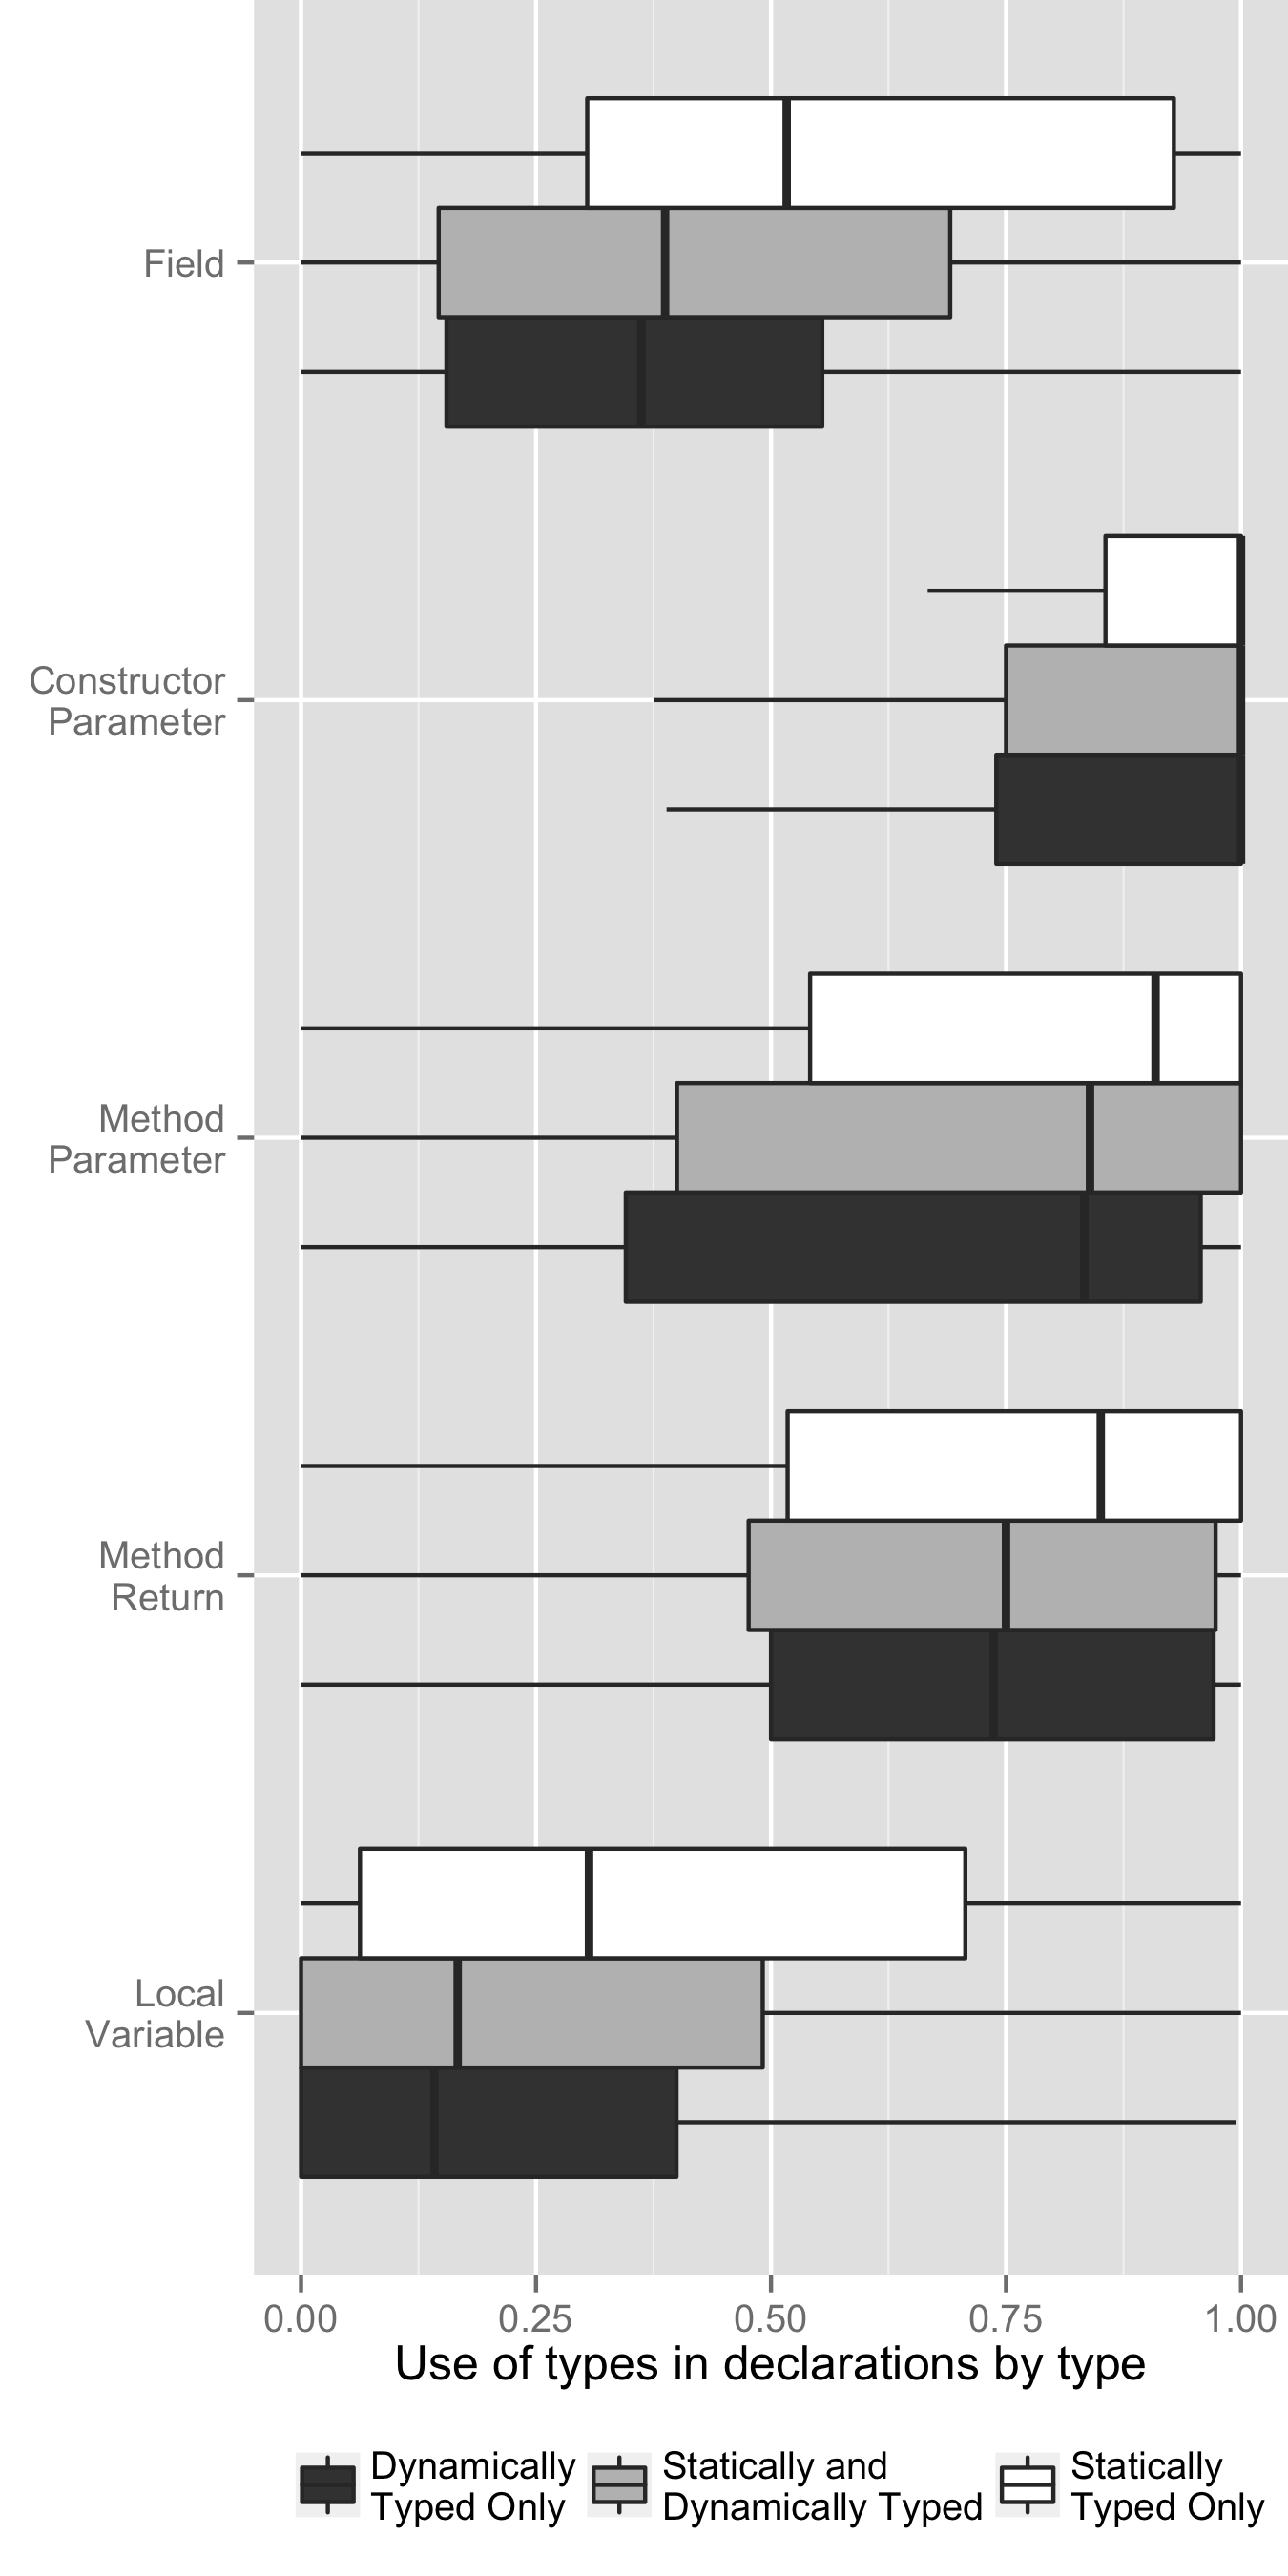
\includegraphics[width=0.7\textwidth]{../aosd_2014/analysis/result/background/comparison/boxplots/6_declarations_by_type.png} 
\vspace{0.1cm}
\renewcommand{\arraystretch}{1.2}


\begin{tabular}{|c|c|c|c|c|c|}
\hline
\cell{Declaration Type}						& \cell{Background}	& N		& Mean		& Median	& \cell{std. dev.}\\
\hline
\hline
{}												& Static			& 782	& 0.56		& 0.52 		& 0.35\\			 
Field											& Both				& 3183	& 0.43		& 0.39 		& 0.34\\			 
{}												& Dynamic			& 2035	& 0.38		& 0.36 		& 0.29\\
\hline								 			
\multirow{3}{*}{\cell{Constructor\\Parameter}}	& Static			& 224	& 0.83		& 1.00 		& 0.33\\			 
												& Both				& 991	& 0.80		& 1.00 		& 0.35\\			 
												& Dynamic			& 455	& 0.80		& 1.00 		& 0.34\\			 
\hline								
\multirow{3}{*}{\cell{Method\\Parameter}}		& Static			& 662	& 0.73		& 0.91 		& 0.34\\			 
												& Both				& 2694	& 0.67		& 0.84 		& 0.36\\			 
												& Dynamic	 		& 1511	& 0.65		& 0.83 		& 0.37\\	
\hline						 			
\multirow{3}{*}{\cell{Method\\Return}}			& Static			& 764	& 0.73		& 0.85 		& 0.30\\			 
												& Both				& 3205	& 0.66		& 0.75 		& 0.32\\			 
												& Dynamic	 		& 1912	& 0.68		& 0.74 		& 0.29\\ 
\hline											
\multirow{3}{*}{\cell{Local Variable}}			& Static			& 798	& 0.39		& 0.31 		& 0.36\\			 
												& Both				& 3230	& 0.28		& 0.17 		& 0.32\\			 
												& Dynamic			& 1817	& 0.25		& 0.14 		& 0.30\\ 
\hline
\end{tabular}
\caption{Usage of types by declaration type and programmer background}
\label{fig:background_boxplot_type}
\end{figure}





\FloatBarrier

The results reported in this section suggest a positive answer for Question Q3, i.e, programmers use types differently depending on their background.
This difference is larger when comparing those projects of the \emph{Static} group with projects of the other groups.
These results are statistically strong,  but should be generalized with care.
The detailed results reported by the Tukey HSD test reveal many exceptions, specially in the comparison between the groups comprising the projects of those programmers who have at least one dynamically typed language in their portfolio, \emph{Static and Dynamic} and \emph{Dynamic Only}.
This comparison reveals that, for all kinds and visibilities of declarations, the difference is either not significant or small.


\begin{figure}[ht]
\centering 
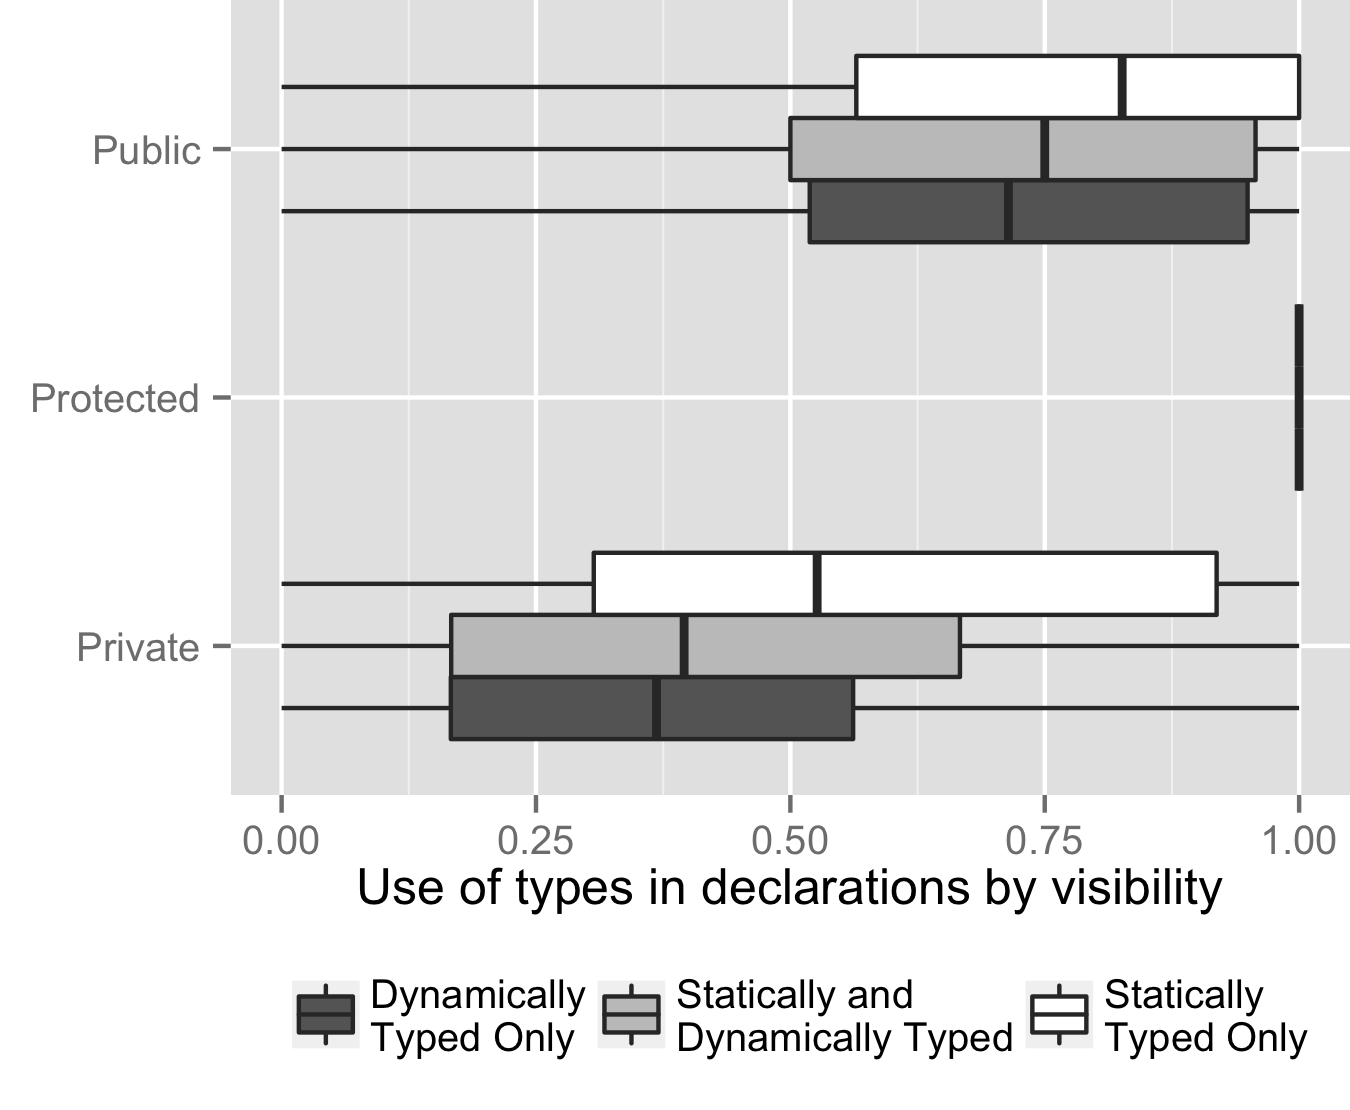
\includegraphics[width=0.7\textwidth]{../aosd_2014/analysis/result/background/comparison/boxplots/23_declarations_by_visibility.png} 
\vspace{0.1cm}
\renewcommand{\arraystretch}{1.2}


\begin{tabular}{|c|c|c|c|c|c|}
\hline
\cell{Declaration Type}						& \cell{Background}	& n		& mean		& median	& \cell{std. dev.}\\
\hline
\hline
{}												& Static			& 757 	& 0.73		& 0.83 		& 0.29\\			 
Public											& Both				& 3191	& 0.68		& 0.75 		& 0.30\\			 
{}												& Dynamic			& 1904	& 0.69		& 0.71 		& 0.27\\
\hline								 								    	    		    		    						
\multirow{3}{*}{\cell{Protected}}				& Static			& 287 	& 0.92		& 1.00 		& 0.20\\			 
												& Both				& 1275	& 0.94		& 1.00 		& 0.18\\			 
												& Dynamic			& 825 	& 0.93		& 1.00 		& 0.20\\			 
\hline																    	    		    		    					
\multirow{3}{*}{\cell{Private}}					& Static			& 787 	& 0.56		& 0.53 		& 0.34\\			 
												& Both				& 3196	& 0.43		& 0.40 		& 0.33\\			 
												& Dynamic	 		& 2040	& 0.38		& 0.37 		& 0.28\\	
\hline						 			
\end{tabular}
\caption{Usage of types by declaration visibility and programmer background}
\label{fig:background_boxplot_visibility}
\end{figure}	

\FloatBarrier



\begin{table}[h!]
\centering{}%
\renewcommand{\arraystretch}{1.2}

\caption{Tukey Honest Significant Differences Test results for the comparison between the usage of types by declaration type and programmers background}
\begin{tabular}{|c|c|c|c|}
\hline 
{}                              & Declaration Type    & p     & Difference  \\
\hline 
\hline 
\multirow{5}{*}{\cell{Static and Dynamic\\vs.\\Static}} & Field         & 0    & (-0.17, -0.07) \\ \cline{2-4}
                              & Constructor Parameter & 1.0  & (-0.12,  0.06) \\ \cline{2-4}
                              & Method Parameter    & 0    & (-0.11, 0.00)  \\ \cline{2-4}
                              & Method Return     & 0    & (-0.11, -0.01) \\ \cline{2-4}
                              & Local Variable    & 0    & (-0.15, -0.05) \\ 
\hline 
\hline

\multirow{5}{*}{\cell{Dynamic\\vs.\\Static}}        & Field         & 0    & (-0.23, -0.12) \\ \cline{2-4}
                              & Constructor Parameter & 0.99 & (-0.12,  0.07) \\ \cline{2-4}
                              & Method Parameter    & 0    & (-0.14, -0.02) \\ \cline{2-4}
                              & Method Return     & 0.01 & (-0.10,  0.00) \\ \cline{2-4}
                              & Local Variable    & 0    & (-0.18, -0.07) \\ 
\hline 
\hline
\multirow{5}{*}{\cell{Static and Dynamic\\vs.\\Dynamic}}  & Field         & 0    & ( 0.01,  0.08) \\ \cline{2-4}
                              & Constructor Parameter & 1.00 & (-0.07,  0.06) \\ \cline{2-4}
                              & Method Parameter    & 0.84 & (-0.02,  0.06) \\ \cline{2-4}
                              & Method Return     & 0.94 & (-0.05,  0.02) \\ \cline{2-4}
                              & Local Variable    & 0.12 & (-0.00,  0.06) \\ 
\hline 
\end{tabular}
\label{tab:background_utest_type}
\end{table}
      
\begin{table}[h!]

\FloatBarrier

\centering{}%
\renewcommand{\arraystretch}{1.2}
\caption{Tukey Honest Significant Differences Test results for the comparison between the usage of types by declaration visibility and programmers background}
\begin{tabular}{|c|c|c|c|}
\hline 
{}                              & Declaration Visibility  & p     & Difference \\
\hline 
\hline 
\multirow{3}{*}{\cell{Static and Dynamic\\vs.\\Static}}   & Public          & 0.00  & (-0.10, 0.00) \\ \cline{2-4}
                              & Protected         & 1.00  & (-0.07,  0.09)  \\ \cline{2-4}
                              & Private         & 0.00  & (-0.18, -0.08)  \\ 
\hline 
\hline

\multirow{3}{*}{\cell{Dynamic\\vs.\\Static}}        & Public          & 0.01  & (-0.10,  0.01)  \\ \cline{2-4}
                              & Protected         & 1.00  & (-0.08,  0.09)  \\ \cline{2-4}
                              & Private         & 0.00  & (-0.23, -0.13)  \\ 
\hline 
\hline
\multirow{3}{*}{\cell{Static and Dynamic\\vs.\\Dynamic}}  & Public          & 0.98  & (-0.04,  0.03)  \\ \cline{2-4}
                              & Protected         & 1.00  & (-0.05,  0.06)  \\ \cline{2-4}
                              & Private         & 0.00  & ( 0.02,  0.09)  \\ 
\hline 
\end{tabular}
\label{tab:backgorund_utest_visibility}
\end{table}



\clearpage

% PROJECT MATURITY
\section{Project Size, Age and Number of Commits\label{sec:results-maturity}}
This section investigates whether programmers use types differently in their code depending on the project characteristics.
We analyze three project metrics: age, number of lines of code and number of commits.
% The latter measures the level of activity of the project.
We start by analyzing the correlation between these metrics and the relative use of types in declarations by type and visibility.
The Spearman rank correlation coefficient is used for this purpose.
This coefficient, which ranges from -1 to 1, is a measure of the dependence between two variables.
A positive value means that two variables are correlated, i.e, as the value of one grows, so does the value of the other.
A negative value means an inverse correlation.
Values close to 1 or -1 indicate very strong relationships and values above 0.5 or below -0.5 can be considered strong correlations.

\begin{table}[h!]

\centering{}%
\caption{Spearman Correlation between the usage of types and the size, age and number of commits of projects}
\begin{tabular}{|c|c|c|c|c|}
\hline 
Declaration Type/Visibility & Size    & Age & Commits\\
\hline 
\hline 
Field           &  0.221  & -0.063  &  0.153  \\ \hline
Constructor Parameter   & -0.072  & -0.132  & -0.053  \\ \hline
Method Parameter      & -0.123  & -0.079  & -0.004  \\ \hline
Method Return       & -0.071  &  0.168  & -0.027  \\ \hline
Local Variable        &  0.057  & -0.049  &  0.112  \\ 
\hline       
\hline     
Public            & -0.063  &   0.119 & -0.024  \\ \hline
Protected         & -0.286  &  -0.020 & -0.165  \\ \hline
Private           &  0.213  &  -0.068 &  0.160  \\ \hline
\end{tabular}
\label{tab:all_correlation_maturity}
\end{table}	

Table \ref{tab:all_correlation_maturity} shows the Spearman correlation coefficient between the usage of types and the age, size and number of commits of a project.
Most of values in this table are close to 0.
There are a few coefficient values which could indicate a relationship, such as \emph{Size} vs. \emph{Protected} or \emph{Commits} vs. \emph{Private}, but these relationships are still considerably weak.
All in all, these values do not seem to suggest any direct relationship between these metrics and the usage of types.

The lack of correlation between the relative usage of types and these metrics does not necessarily imply that they have no influence on the usage of types.
A possibility is that this influence appears only in the most mature projects, where the values of all of these three metrics are large enough.
In order to determine whether this is true, we conduct now a comparison between mature projects and the rest of the dataset.
We define a mature project as a project that is 100 days old or more and has, at least, 2KLoC and 100 commits.
These numbers were defined by manually inspecting our dataset and finding that there are popular and mature projects that barely exceed these three metrics.
According to our criteria, there are 223 mature projects in our dataset, which are characterized in Table \ref{tab:mature_dataset_characterization}.


\begin{table}[h!]

\centering{}%
\renewcommand{\arraystretch}{1.2}

\caption{Descriptive statistics for mature projects}
\begin{tabular}{|c|c|c|c|c|c|}
\hline
{}    & Mean  & Median  & Std. Dev. & Max & Total   \\
\hline
\hline
Size (LoC)  & 9947  & 5627 & 14594  & 149933  & 2218189 \\ \hline
Commits     & 487   & 213    & 800   & 6545   & 108583  \\ \hline
Age (Days)  & 600   & 574  & 350   & 1469   & 133697  \\ \hline
\end{tabular}
\label{tab:mature_dataset_characterization}
\end{table}

Figures \ref{fig:size_boxplot_type}  and \ref{fig:size_boxplot_visibility} show the box plots for the usage of types in mature projects and others by declaration type and visibility respectively.
The ANOVA test reported a \emph{p} value equal to 0.0518 for this analysis, which implies that there are no treatments that are significantly different from each other.
Because of this, we do not report the results for the Tukey HSD test.
This result, along with the very low correlation coefficients reported in Table \ref{tab:all_correlation_maturity}, implies that the answer for Question Q4 is negative.
There is no significant difference in how programmers type declarations in mature projects compared to declarations in other projects.

\begin{figure}[h!]
\centering 
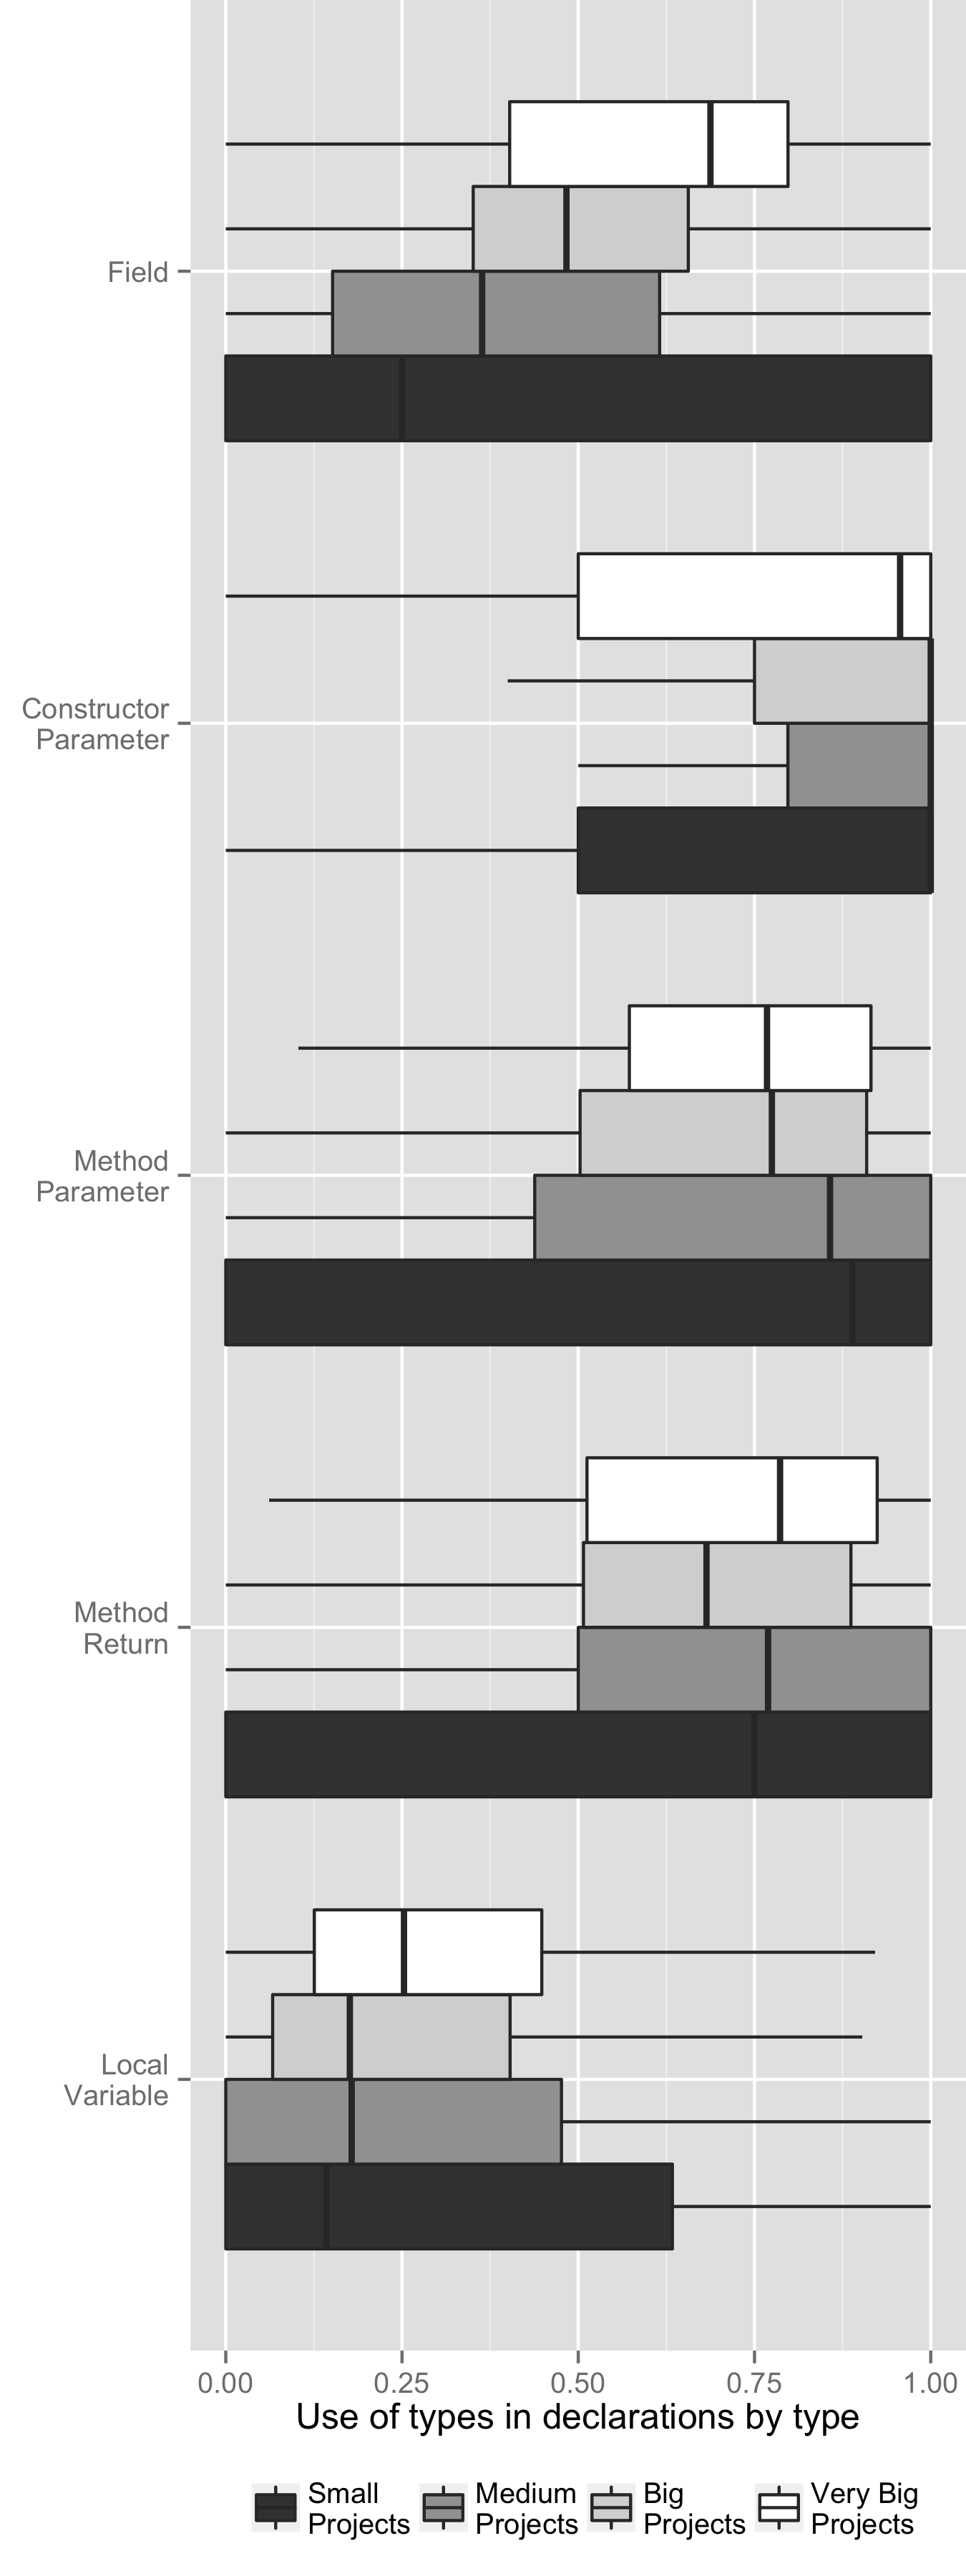
\includegraphics[width=0.7\textwidth]{../aosd_2014/analysis/result/size/comparison/boxplots/6_declarations_by_type.png} 
\vspace{0.1cm}
\renewcommand{\arraystretch}{1.2}


\begin{tabular}{|c|c|c|c|c|c|}
\hline
\cell{Declaration Type}	& \cell{Project Type}& n	& mean	& median	& \cell{std. dev.}\\
\hline
\hline
\multirow{2}{*}{Field}		& Mature		& 221 	& 0.53 		& 0.48	& 0.27 \\
							& Other			& 5779	& 0.43 		& 0.39	& 0.33 \\                
\hline                																								
Constructor					& Mature		& 172 	& 0.83 		& 1.00	& 0.30 \\                
Parameter	 				& Other			& 1498	& 0.80 		& 1.00	& 0.35 \\                
\hline																								
Method						& Mature		& 222 	& 0.69 		& 0.78	& 0.29 \\                
Parameter      				& Other			& 4645	& 0.67 		& 0.86	& 0.37 \\                
\hline																								
Method		         		& Mature		& 222 	& 0.72 		& 0.79	& 0.24 \\                
Return						& Other			& 5659	& 0.68 		& 0.75	& 0.32 \\                
\hline																								
Local						& Mature		& 223	& 0.32 		& 0.22	& 0.28 \\                
Variable					& Other			& 5622 	& 0.29 		& 0.17	& 0.32 \\                
\hline																								
\end{tabular}
\caption{Usage of types in projects by declaration type and project maturity}
\label{fig:size_boxplot_type} 
\end{figure}


\begin{figure}[h!]
\centering 
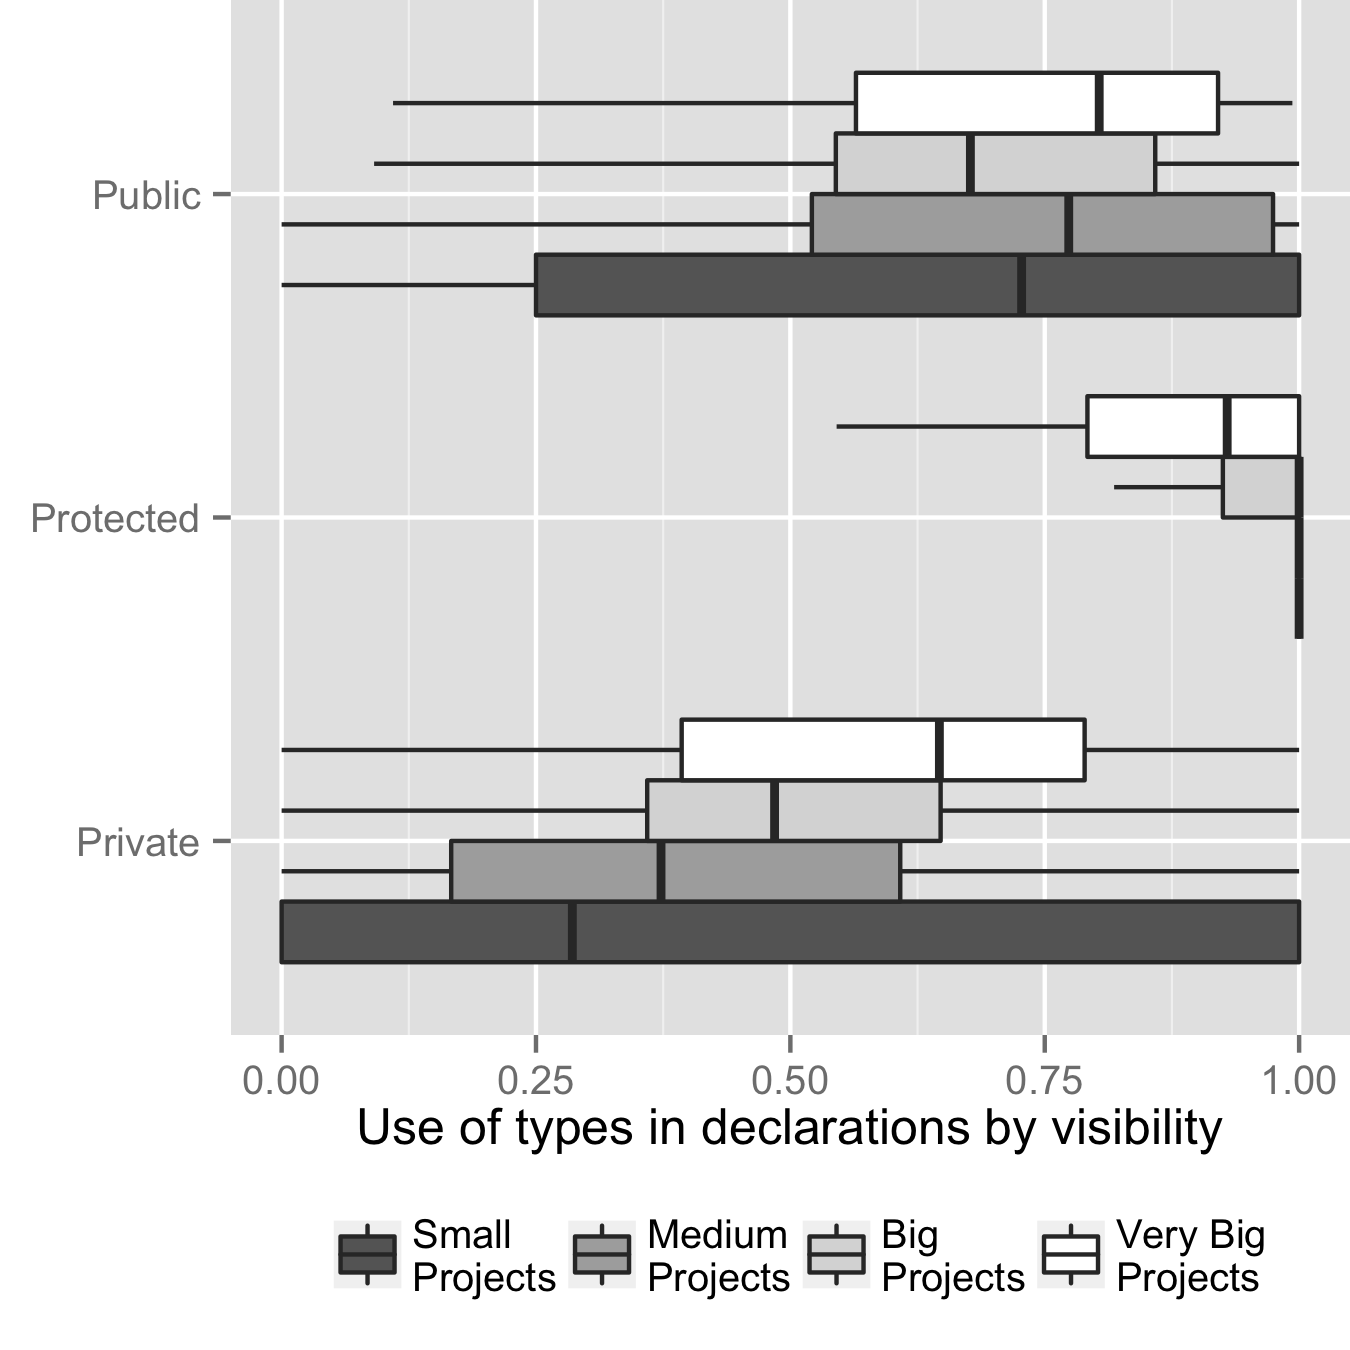
\includegraphics[width=0.7\textwidth]{../aosd_2014/analysis/result/size/comparison/boxplots/23_declarations_by_visibility.png} 
\vspace{0.1cm}
\renewcommand{\arraystretch}{1.2}


\begin{tabular}{|c|c|c|c|c|c|}
\hline
\cell{Declaration Type}			& \cell{Project Type}	& n		& mean		& median	& \cell{std. dev.}\\
\hline
\hline
\multirow{2}{*}{\cell{Public}}		& Mature				& 223 	& 0.72		& 0.76 		& 0.24\\
{}									& Other					& 5629	& 0.69		& 0.75 		& 0.29\\			 
\hline								 							  	  			  			  							
\multirow{2}{*}{\cell{Protected}}	& Mature				& 183 	& 0.88		& 1.00 		& 0.21\\			 
									& Other					& 2204	& 0.94		& 1.00 		& 0.19\\			 
\hline															  	  			  			  						
\multirow{2}{*}{\cell{Private}}		& Mature				& 221 	& 0.53		& 0.48 		& 0.26\\			 
									& Other					& 5802	& 0.43		& 0.40 		& 0.32\\			 
\hline						 			
\end{tabular}
\caption{Usage of types in projects by declaration visibility and project maturity}
\label{fig:size_boxplot_visibility}
\end{figure}	




% \begin{table}[h!]
% \centering{}%
% 
% \caption{Tukey Honest Significant Differences Test results for the comparison between the usage of types by mature projects and others}
% \begin{tabular}{|c|c|c|}
% \hline 
% Declaration Type/Visibility     & p & Difference \\
% \hline 
% \hline 
% Field                  & 0.0000 & (0.053,0.173) \\ \hline
% Constructor Parameter  & 0.3203 & (0.000,0.000) \\ \hline
% Method Parameter       & 0.0794 & (-0.051,0.002) \\ \hline
% Method Return          & 0.9373 & (-0.031,0.051) \\ \hline
% Local Variable         & 0.0002 & (0.012,0.078) \\ \hline
% \hline 
% Public    & 0.8540  & (-0.031,0.045)  \\ \hline
% Private   & 0.0000  & (0.000,0.000)   \\ \hline
% Protected & 0.0000  & (0.055,0.169)   \\ 
% \hline 
% \end{tabular}
% \label{tab:size_utest_type+visibility}
% \end{table}	


% FREQUENCY OF CHANGES
\section{Frequency of changes\label{sec:results-changes}}
This section investigates whether programmers prefer to type their declarations in frequently changed code or not.
Only the mature projects defined in the previous section are considered since we would not be able to obtain meaningful results from small and young projects.

We found that in most of the mature projects programmers prefer untyped declarations in frequently changed code.
We calculated the Spearman correlation coefficient between the frequency of changes of a file and the usage of types in that file for all mature projects.
In projects where types are used more often in frequently changed files, this coefficient is positive, and negative when untyped declarations are preferred.
Figure \ref{fig:change_spearman} displays the cumulative distribution of this coefficient across the mature projects dataset.
It shows that 65\% of them present a negative Spearman correlation coefficient and that almost half of these present strong correlations, i.e., inferior to -0.5.
On the other hand, only 10\% of the mature projects present strong positive correlations.

\begin{figure}[h]
\centering 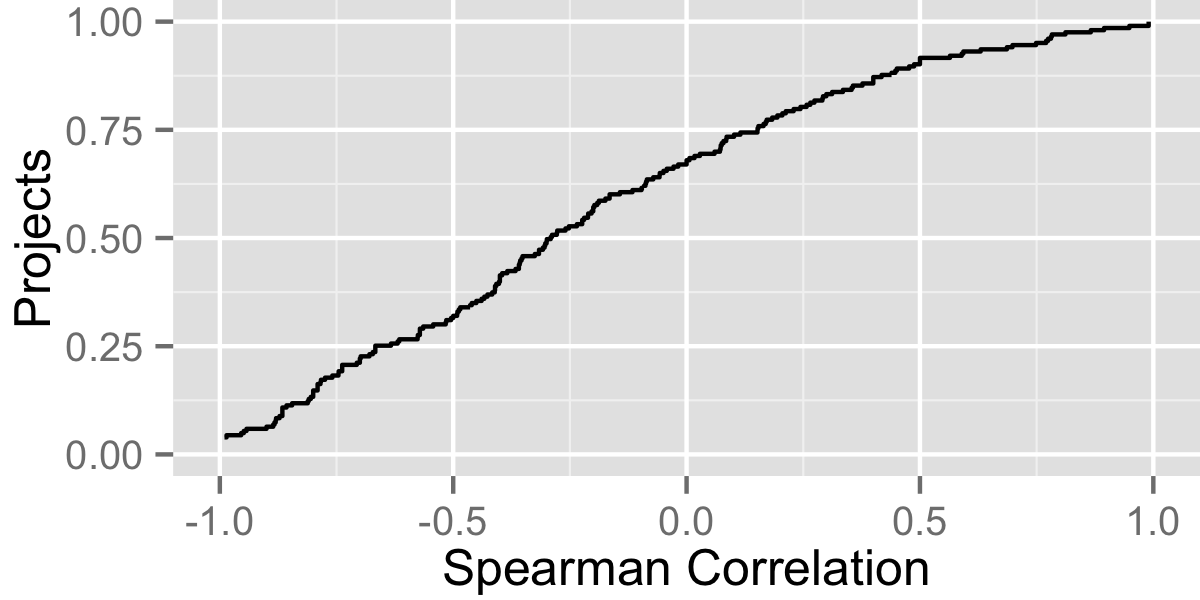
\includegraphics[width=0.6\textwidth]{../aosd_2014/analysis/result/change_commits_distribution.png} 
\caption{Spearman ranking for the correlation between frequency of changes of files and the usage of types in mature projects}
\label{fig:change_spearman} 
\end{figure}
















%
% DISCUSSION
%
\chapter{Discussion\label{discussion}}

This chapter is split in two sections.
We try and answer the research questions in Section \ref{questions-answers}.
In Section \ref{threats}, we discuss the threats to the validity of this study.

\section{Research Questions\label{questions-answers}}
In this section, we discuss the results of our study in the light of the research questions proposed in Section \ref{questions}.
Although we were able to obtain a good understanding of the usage of types in different contexts, the cause for such results is still unclear in many of them.
We provide several hypotheses with the goal of identifying future research topics that can provide more detailed insights about such causes.

% Q1
\subsection*{Q1: Do programmers use types more often in the interface of their modules?\label{discussion-q1}}
The analysis of the usage of types by kind and visibility of declarations, presented in Sections \ref{sec:results-type} and \ref{sec:results-visibility}, provides clear evidence that the answer for Q1 is affirmative.
Private declarations are typed less often than protected and public declarations.
Also, fields, methods and constructors are typed more often than local variables.
Although fields are significantly less typed than methods and constructors, this can be explained by the fact that most fields are declared privately as shown in Section \ref{dataset}.
In Groovy, similar to what happens with Java, interactions with fields of other modules usually happen through accessor methods.

While it is clear that module definitions are typed more often, the cause for such phenomena is still open to discussion.
We believe that the main motivation for this is the implicit documentation provided by types.
In these scenarios, types provide useful hints about the behavior of modules (\cite{Curtis1987}) and define pre and post condition of contracts
\cite{Meyer88, Meijer04, Wadler04, Plosch97, Flanagan2006, Furr09}.
Users of a well defined module learn how to use it faster and do not need to read its implementation to understand how to use it.
Programmers may consider that delicate contracts, such as those defined by protected methods, should be well documented and thus are typed more often.

Constructor parameters and protected declarations are always the elements typed most often.
In addition, the analyses of different contexts, i.e, main and test classes, mature and non-mature projects and programmers' backgrounds, show no significant difference in the usage of types.
This reveals that the presence of these particular declarations is considered by programmers as a more important factor in their choice whether to type a declaration than these contexts.
We hypothesize that programmers consider documentation more important in these elements.
Constructors usually define the dependencies of an object, at least for its creation.
In addition, they might be the first element that a programmer interacts with when dealing with a new module.
Protected declarations are often used as a means to delegate the implementation of a method to subclasses, which requires a well defined contract so the superclass can work properly.
Moreover, they give subclasses and other classes in the same package access to internal elements of a class, forming a tightly coupled relationship (\cite{Chidamber94}).


We can also speculate that declarations that are not part of a module definition, which are local variables and those with private visibility, require less documentation and thus are typed less often.
Programmers can easily find all the references to these elements.
Local variables are only used inside the block of code where they are declared, while all the references to elements declared privately are in the same file.
This makes it easier for a programmer to infer the type of such a declaration even when it is not explicitly defined.

Documentation may not be the only reason why programmers type declarations in modules interfaces.
We can think of at least two other reasons.
First, a programmer might type a declaration so that he or she can get code assistance from the development environment.
For example, typing the declaration of a method parameter allows the development environment to provide code completion for that parameter inside the method.
Another possibility is that, even though Groovy is actually a dynamically typed language, programmers might type their declarations thinking that the compiler will check for type errors, which would lead to safer interactions between modules.

% TODO
% Hanenberg13
% Our analysis suggest that programmers are aware of these tradeoffs and consider them when choosing whether or not to type their declarations.
% In potentially simpler scenarios, such as scripts and tests, we show a lower usage of types.
% Conversely, programmers type the interface of their modules very often, probably as a means to document their codem which potentially improves the development time in more complex scenarios.

% Q2
\subsection*{Q2: Do programmers use types less often in test classes and scripts?\label{discussion-q2}}
There are notable differences between the usage of types in either test classes or scripts and the main classes of a program.
Sections \ref{sec:results-tests} and \ref{sec:results-scripts} show that, in these scenarios, programmers use types less often.
If we are right about our hypothesis that programmers type their modules as a means to document their code, this could explain this less frequent use of types.
Scripts and test classes are usually not designed as reusable modules.
Test classes have the sole goal of verifying a program's functionality and not interfering with it while scripts cannot be instantiated or referenced by other modules.
In these scenarios, programmers might perceive documentation as less important.
It is curious however that test code itself is usually perceived as a form of documentation (\cite{Beck03,Meyerovich13}).
Because of this, we were expecting programmers to actually use more types in test classes as a means to improve the documentation they provide.
Perhaps, although programmers use test classes as documentation, they might not write them with this goal in mind.

An alternative explanation for the fact that scripts and tests are typed less frequently is that most of them are probably simpler than main classes.
As found in the recent work of Hanenberg et al.(\cite{Hanenberg13}), untyped code potentially has a positive impact on the development time of easier tasks.
In such case, programmers might not type their declarations in scripts or test classes since this would allow them to finish their tasks faster.

% Q3
\subsection*{Q3: Does the experience of programmers with other languages influence their choice for typing their code?\label{discussion-q3}}
The analysis presented in Section \ref{sec:results-background} indicates that the answer for Question Q3 is affirmative.
The choice for using types on a language with optional typing, such a Groovy, is in fact influenced by the programmers' experience with other languages.
In general, those programmers who have only statically typed languages in their portfolio type more often than the others.
However, the two groups with projects written by programmers who have either statically and dynamically typed languages or only dynamically typed languages are very similar in most cases.
Apparently programmers who develop in an "untyped" language get used to the lack of types, leading them to declare types less often.
This hypothesis supports the work of Daly et al. which suggests that programmers have ways of reasoning about types that compensate for the lack of static type information (\cite{ruby_vs_druby}).
% Our analysis of the programmers' backgrounds supports this argument.
% It shows that those programmers who have worked with dynamically typed languages in fact use types less often.

% Q4
\subsection*{Q4: Does the size, age or level of activity  of a project have any influence on the usage of types?\label{discussion-q4}}
We initially believed that, as these metrics grow, the maintenance of projects becomes more difficult, leading programmers to use more types as a means to make code more readable.
However, the analysis presented in Section \ref{sec:results-maturity} shows no evidence of such behavior.
We consider two hypotheses in order to explain these results.
First, the considered metrics might not actually correlate to the need for maintenance of projects.
Second, even if these metrics are a good indicative of the necessity of better maintainability, once projects start growing and aging, programmers might not have the opportunity or desire to make their code more maintainable.

% Q5
\subsection*{Q5: In frequently changed code, do developers prefer typed or untyped declarations?\label{discussion-q5}}
In frequently changed code, there are arguments in favor and against using types.
Since types act as documentation, programmers might use them to make code more maintainable and easier to change  (\cite{should_your_specification_language_be_typed}).
On the other hand, untyped code is simpler and can potentially be changed faster (\cite{gradual_typing}).
The results presented in Section \ref{sec:results-changes} however suggests that the latter is considered more often than the former.

In most projects, the usage of untyped declarations grows as the frequency of changes in a file increases.
Apparently, programmers understand that untyped code makes maintenance tasks easier.
One can argue that the causal relationship is the opposite, i.e., these files have to be changed more often due to the use of untyped declarations.
However, it is very unlikely that programmers would not notice that untyped declarations would be causing such problems and would not add types to those declarations in order to fix them.


\section{Threats to Validity\label{threats}}
In this section, we discuss potential threats to validity of our study. As usual, we have arranged possible threats in two categories, internal and external validity (\cite{Wohlin2012}). 

\subsection*{Internal Validity}
Perhaps the most relevant internal threat to our study is that in a large scale empirical study such as ours, there might be many confounds which are difficult to identify.
In Section \ref{sec:results-background} we consider that the GitHub portfolio of a programmer represents well his experience with other languages and type systems, but this might not be true for all programmers.
They may have projects in their portfolio that they have not worked on or projects hosted elsewhere written in other languages.
There is also the possibility of a programmer having multiple GitHub accounts with different languages in each one, causing such a programmer to be measured twice with different inferred backgrounds.
Due to the large number of programmers considered in our study, we expect these special cases not to have a large influence on the results.

There are other factors that might have influenced programmers besides the ones considered in this study.
Some frameworks require programmers to use typed or untyped declarations in some cases.
For example, we found that the data collected in test classes is biased by the fact that popular testing frameworks, such as JUnit, require test methods to have their returns declared as \emph{void}.
There might be other similar cases that we are not aware of.
% In addition, the type of application developed by these programmers might have influenced their choices.
% In addition to that, the programmers' background, which we have shown to have influence over programmers, might interfere with the analysis of other influencing factors.

\subsection*{External Validity}
Although we have analyzed a very extensive number of Groovy projects, it cannot be said that we have covered all possible scenarios.
By manually inspecting our dataset, we could find only a few projects with characteristics of software developed inside an organization.
Most of them were developed by small groups of people or open source communities.
Enterprise projects are probably hosted privately on GitHub or in private servers, and hence unavailable to us.

The behavior observed for Groovy projects can be very different in other languages.
Most languages are not like Groovy and feature either static or dynamic typing, forcing programmers to choose a single typing strategy for all scenarios in a single project.
Even a language with a hybrid typing paradigm might implement different strategies which will be perceived differently by the programmers of that language.
Finally, the tools used to code in a given language might influence programmers to chose different type strategies.











%
% CONCLUSION AND FUTURE WORK
%
\chapter{Conclusions and Future Work\label{conclusion}}

In this chapter, we show the main conclusions of this study in Section \ref{sec:conclusion} and describe future work in Section \ref{sec:future}.

\section{Conclusions\label{sec:conclusion}}
Type systems is an important topic in software engineering and is becoming even more popular with the growing adoption of dynamically typed languages, such as JavaScript and Ruby.
While using types potentially leads to more reliable and maintainable code, untyped programs might be faster to write and easier to change.
This dissertation presented a study with the goal of finding how programmers of an optionally typed language perceive these tradeoffs.
Through the large scale analysis of the source code of 6638 projects written in Groovy we were able to find in which situations programmers preferred the usage of types or not.
We found the following results:

\begin{itemize}
	\item \emph{Groovy programmers type declarations that define the interface of modules more often than other declarations.} 
While public and protected declarations were typed very frequently, most private declarations and declarations of local variables were not typed. We also found that protected declarations and declarations of constructors, which we believe to be extremely important elements of a module definition, were almost always typed.

	\item \emph{Types are used differently in test classes and script files.}  We observed a much higher usage of types in functional classes and class files than in these scenarios.

	\item \emph{A programmer's background influences the choice of programmers whether to use types or not.} Those programmers who have developed in at least one dynamically typed language use types less frequently than those who have only worked with statically typed languages.
	
	\item \emph{Apparently, there is no influence of the size, age or level of activity of a project on how programmers use types.} We have not found any correlation between these variables and the usage of types. We also analyzed the usage of types in projects considered mature, where all of these variables had high values, and found no significant difference to other projects.

	\item \emph{Untyped declarations are more popular in frequently changed files.} In most projects, the files that change more frequently are also those files with a lower usage of types.
\end{itemize}

We believe that these results are valuable to developers of programming languages and development tools, who can base their designs on real user data.
Also, programmers can understand the tradeoffs between using or not types in their projects.
Our results provide a different point of view and complement previous studies, which analyzed typing strategies through the use of controlled experiments. 
We hope that the questions raised in our discussion can inspire other researchers to analyze our findings in more detail.

\section{Future Work\label{sec:future}}
\subsection*{Measuring the impact of compile, runtime and unit test error messages on maintenance time}
In future work we want to conduct controlled experiments and qualitative studies in order to evaluate some of our results in more detail.
In particular, we have started a new study with the goal of comparing the productivity of developers on maintenance tasks of statically typed software and unit tested dynamically typed software.
Our hypothesis is that, given the proper set of automated tests, dynamically typed languages can lead to systems which are as robust and maintainable as those written with statically typed languages.

Our first experiment compares the development time of developers fixing a few type errors.
They are given either compiler error messages, runtime exceptions or unit test error messages.
Preliminary results show that programmers develop their tasks much faster when dealing with compiler error messages than with runtime exceptions.
However, there is no significant difference between those developers dealing with compiler error messages and unit test error messages.
These results lead us to believe that, in fact, unit tests make up for the lack of type checking.

\subsection*{ERA: An Elastic Framework for Repository Analysis on the Cloud}
Another work in progress is a framework for the static source code analysis of massive datasets called Elastic Repository Analysis - ERA\footnote{http://github.com/carlosgsouza/ERA}.
This framework is based on the artifacts we built to analyze the Groovy projects in this study.
ERA will help researchers retrieve large numbers of projects from GitHub and process these projects quickly on the cloud using Amazon Web Services.
It will take care of downloading and storing huge amounts of projects and managing a large set of computing instances to process such projects.


\subsection*{Groovonomics: Sharing the results with the Groovy community}
One of the main contributions of this dissertation is to allow programming language and tools developers to base their designs on precise and real user data.
In particular, we believe that the Groovy community can greatly benefit from these results.
However, in order to effectively share these results with them, we need to generate a simpler representation of our data so they can be understood by people outside the academic community.
We are working on an website called \emph{groovonomics}, which will display such results in the form of infographics, making them easier to be absorbed.

% In our discussion, in Section \ref{discussion}, we avoided providing definitive answers for what caused the behavior we found in our analysis.
% Instead, we raised many hypothesis to explain these results.
% It is difficult however to state whether these hypothesis make sense or not.
% In order to overcome this uncertainty, we are planning a series of controlled and qualitative studies which will complement the findings in this study in order to validate or reject these hypothesis.




% \ppgccbibliography{bibfile}
\bibliographystyle{abbrvnat}
\renewcommand{\bibfont}{\normalsize}
\begin{thebibliography}{}


\bibitem[Beck (2003)]{Beck03}
K. Beck.  Test-driven development: by example. Addison-Wesley Professional, 2003.

\bibitem[Bruce (2002)]{Bruce2002}
K. Bruce. Foundations of object-oriented languages: types and semantics. The MIT Press, 2002.

\bibitem[Bruch et. al.(2009)]{bruch2009learning}
M. Bruch, M. Monperrus, and M. Mezini. Learning from examples to improve code completion systems. In Proceedings of the International Symposium on the Foundations of Software Engineering (FSE), 213-222, 2009.

\bibitem[Cardelli (1996)]{type_systems}
L. Cardelli. Type systems. ACM Computing Surveys, 28(1), 263-264, 1996.

\bibitem[Chang et. al.(2011)]{jit}
M. Chang, B. Mathiske, E. Smith, A. Chaudhuri, A. Gal. M. Bebenita, C. Wimmer, and M. Franz. The impact of optional type information on jit compilation of dynamically typed languages. SIGPLAN Notices, 47(2), 13-24, 2011.

% Coupling is high for inheritance
% interaction coupling, component coupling and inheritance coupling
\bibitem[Chidamber et. al.(1994)]{Chidamber94}
S. Chidamber and C. Kemerer. A metrics suite for object oriented design. IEEE Transactions on Software Engineering, 20(6), 476-493, 1994.

% \bibitem[Cohen (1988)]{Cohen88}
% J. Cohen. Statistical power analysis for the behavioral sciences (2nd ed.). Hillsdale, NJ: Lawrence Erlbaum, 1988.

\bibitem[Curtis (1987)]{Curtis1987}
B. Curtis. Five paradigms in the psychology of programming. MMC, 1987.

\bibitem[Daly et. al.(2009)]{ruby_vs_druby}
M. Daly, V. Sazawal, and  J. Foster. An empirical study of static typing in ruby. In Proceedings of the Workshop on Evaluation and Usability of Programming Languages and Tools (PLATEAU), 2009.

\bibitem[ERA(2014)]{era}
ERA - Elastic Repository Analysis. http://github.com/carlosgsouza/ERA

\bibitem[Fenton(1998)]{Fenton1998}
N. Fenton and S. Pfleeger. Software metrics: a rigorous and practical approach. PWS Publishing Co., 1998.

%Traditional static type systems are very effective for verifying basic interface specifications
\bibitem[Flanagan (2006)]{Flanagan2006}
C. Flanagan. Hybrid type checking. ACM SIGPLAN Notices. Vol. 41. No. 1, 2006.

\bibitem[Fowler (2010)]{fowler10}
M. Fowler, Domain-specific languages. Pearson Education, 2010.

\bibitem[Furr et. al.(2009)]{Furr09}
M. Furr et al. Static type inference for Ruby. In Proceedings of the ACM symposium on Applied Computing (ACM SAC), 2009.

% Use of types in interfaces
\bibitem[Gannon (1977)]{Gannon77}
J. Gannon.  An experimental evaluation of data type conventions. Communications of the ACM, 20, 8, 584-595, 1977.

\bibitem[Gray (2008)]{gray08}
K. Gray. Safe cross-language inheritance. In Proceedings of the European Conference on Object-Oriented Programming (ECOOP), pp. 52-75.

\bibitem[Gray (2011)]{gray11}
K. Gray. Interoperability in a scripted world: Putting inheritance \& prototypes together. In Proceedings of Foundations of Object-Oriented Languages (FOOL), 2011.

\bibitem[Gray et. al.(2005)]{gray05}
K. Gray, R. Findler, M. Andflatt. Fine-grained interoperability through contracts and mirrors. In Proceedings of the International Conference on Object-Oriented Programming, Systems, Languages, and Applications (OOPSLA), pp. 231-245, 2005.

\bibitem[Groovy (2013)]{groovy}
Groovy programming language. http://groovy.codehaus.org/. Accessed in 10/10/2013.

\bibitem[Hanenberg (2010)]{experiment_with_purity}
S. Hanenberg, An experiment about static and dynamic type systems: doubts about the positive impact of static type systems on development time. SIGPLAN Notices, 45(10), 22-35, 2010.

\bibitem[Hanenberg et. al.(2013)]{Hanenberg13}
S. Hanenberg, S. Kleinschmager, R. Robbes, E. Tanter, A. Stefik. An empirical study on the impact of static typing on software maintainability. Empirical Software Engineering - An International Journal, 1-48, 2013.

\bibitem[ISO25000(2004)]{Iso2004}
ISO, and IEC FCD. 25000, Software engineering-software product quality requirements and evaluation (SQuaRE) - Guide to SQuaRE. International Organization for Standardization, 2004.

\bibitem[Kirk (1995)]{kirk1995}
R. E. Kirk. Experimental Design: Procedures for the Behavioral Sciences, 3rd edn. Brooks/Cole, Pacific Grove, California, 1995.

\bibitem[Kleinschmager et. al.(2012)]{hanenberg_icpc}
S. Kleinschmager, S. Hanenberg, R. Robbes, and A. Stefik. Do static type systems improve the maintainability of software systems? An empirical study. In Proceedings of the 20th IEEE International Conference on Program Comprehension (ICPC), 153- 162, 2012.

\bibitem[Labovitz (1968)]{labovitz68}
S. Labovitz, Criteria for selecting a significance level: A note on the sacredness of. 05. The American Sociologist 3.3, 220-222, 1968.

\bibitem[Lamport et. al.(1999)]{should_your_specification_language_be_typed}
L. Lamport, and L. Paulson. Should your specification language be typed. ACM Transactions on Programming Languages and Systems, 21(3), 502-526, 1999.

\bibitem[Mayer et. al.(2012)]{mayer2012static}
C. Mayer, S. Hanenberg, R. Robbes, E. Tanter, and A. Stefik. Static type systems (sometimes) have a positive impact on the usability of undocumented software: An empirical evaluation.  Technical Report 20120418-005, 2012.

% Types help on the definition of a contract
\bibitem[Meijer et. al.(2004)]{Meijer04}
E. Meijer and D. Peter. Static typing where possible, dynamic typing when needed: The end of the cold war between programming languages. In Proceedings of the International Conference on Object-Oriented Programming, Systems, Languages, and Applications (OOPSLA), 2004.

\bibitem[Meyer (1988)]{Meyer88}
B. Meyer. Object-oriented software construction, Vol. 2. Prentice hall, 1988.

\bibitem[Meyerovich et. al.(2013)]{Meyerovich13}
L. Meyerovich and A. Rabkin. Empirical analysis of programming language adoption. In Proceedings of the International Conference on Object-Oriented Programming, Systems, Languages, and Applications (OOPSLA), 1-18, 2013.

\bibitem[Milner (1978)]{Milner78}
R. Milner. A theory of type polymorphism in programming. Journal of computer and system sciences 17.3 (1978): 348-375.

\bibitem[Pierce (2002)]{types_and_programming_languages}
B. Pierce. Types and programming languages. MIT press, 2002.

% Unfortunately, dynamically typed programming languages usually do not support the concept of DEC. Therefore we integrated DEC into the programming language Python by using a metaprogramming approach
\bibitem[Plosch (1997)]{Plosch97}
R. Plosch. Design by contract for Python. Proceedings of the Asia Pacific Software Engineering Conference (APSEC), 1997.

\bibitem[Prechelt et. al.(1998)]{Prechelt98}
L. Prechelt and  W. Tichy. A controlled experiment to assess the benefits of procedure argument type checking. IEEE Transactions of Software Engineering, 24(4), 302-312, 1998.

\bibitem[Siek et. al.(2007)]{gradual_typing}
J. Siek, and W. Taha. Gradual typing for objects. In Proceedings of the European Conference on Object-Oriented Programming (ECOOP),  2-27, 2007.

\bibitem[Siek et. al.(2007)]{siek07}
J. Siek, W. Andtaha. Gradual typing for objects. In Proceedings of European Conference on Object-Oriented Programming (ECOOP), 2-27, 2007.

\bibitem[Souza et. al.(2013)]{souza_vem2013}
C. Souza, E. Figueiredo, M. T. Valente. Tipar ou não Tipar? Compreendendo Quais Fatores Influenciam a Escolha por um Sistema de Tipos. In First Brazilian Workshop on Visualization, Evolution and Software Maintenance (VEM), 2013. 

\bibitem[Souza et. al.(2014)]{souza_aosd2014}
C. Souza, E. Figueiredo. How Do Programmers Use Optional Typing? An Empirical Study. In 13th International Conference on Modularity (Modularity), 2014.

\bibitem[Takikawa et. al.(2012)]{takikawa12}
A. Takikawa, T. S. Strickland, C. Dimoulas, S. Tobin-Hochstadt, M. Felleisen. Gradual typing for first-class classes. ACM SIGPLAN Notices. Vol. 47. No. 10. ACM, 2012.

\bibitem[Tiobe Website(2013)]{tiobe}
Tiobe programming community index. http://www.tiobe.com/index.php/content/paperinfo/tpci/index.html. Accessed in 23/09/2013.

\bibitem[Tratt (2009)]{dynamically_typed_languages}
L. Tratt. Dynamically typed languages. Advances in Computers, vol. 77, 149-184, 2009.

\bibitem[Wadler et. al.(2004)]{Wadler04}
P. Wadler and R. Findler. Well-typed programs can't be blamed. Proceedings of the 18th European Symposium on Programming Languages and Systems (ESOP), 1-16, 2009.

\bibitem[Wohlin (2012)]{Wohlin2012}
C. Wohlin et al. Experimentation in software engineering. Springer Publishing Company, 2012.

\end{thebibliography}


\begin{appendices}

% \chapter{ERA: An Elastic Framework for Repository Analysis on the Cloud\label{era}}


\end{appendices}


\begin{attachments}


\chapter{Detailed Results\label{detailed_results}}


\end{attachments}


\end{document}
